\documentclass[a4paper, twoside,openright ,titlepage, 12pt]{report}
\usepackage[english]{babel} % Using babel for hyphenation
\usepackage[utf8]{inputenc}
\usepackage[T1]{fontenc}

\usepackage{amssymb}
\usepackage{graphicx}
\usepackage{amsmath}
\usepackage{epsfig}
%\usepackage{hyperref}
\usepackage{color}
\usepackage{multirow}
\usepackage[parfill]{parskip} % Removes indents
\usepackage[ruled,vlined]{algorithm2e}
\usepackage[most]{tcolorbox}
\usepackage[ ]{titlesec}  % chapter header
\usepackage[toc,page]{appendix}
\usepackage{listings}
\usepackage{enumerate}
\usepackage{subfigure}

%%%APPENDIX
\usepackage[toc,page]{appendix}


%%%%

%%%%%%%%%%%%%%%%%%%%%%%%%%%%% python style
\usepackage[utf8]{inputenc}
\DeclareFixedFont{\ttb}{T1}{txtt}{bx}{n}{9} % for bold
\DeclareFixedFont{\ttm}{T1}{txtt}{m}{n}{9}  % for normal
% Defining colors
\definecolor{deepblue}{rgb}{0,0,0.5}
\definecolor{deepred}{rgb}{0.6,0,0}
\definecolor{deepgreen}{rgb}{0,0.5,0}
\definecolor{mygray}{rgb}{0.5,0.5,0.5}
% Python style for highlighting
\newcommand\pythonstyle{\lstset{
language=Python,
backgroundcolor=\color{white}, %can remove comma for other result
breakatwhitespace=false,         % sets if automatic breaks should only happen at whitespace
breaklines=true,                 % sets automatic line breaking
captionpos=b,
basicstyle=\ttm,
otherkeywords={self},            
keywordstyle=\ttb\color{deepblue},
emph={F_(d):, J_(d):},     
frame=single,	                   % adds a frame around the code
keepspaces=true,                 % keeps spaces in text, useful for keeping indentation of code (possibly needs columns=flexible)
numbers=left,                    % where to put the line-numbers; possible values are (none, left, right)
numbersep=5pt,                   % how far the line-numbers are from the code
numberstyle=\tiny\color{mygray}, % the style that is used for the line-numbers     
emphstyle=\ttb\color{deepred},    
stringstyle=\color{deepgreen},
commentstyle=\color{red}
frame=tb,                         
showstringspaces=false            
}}

% Python environment
\lstnewenvironment{python}[1][]
{
\pythonstyle
\lstset{#1}
}
{}
%%%%%%%%%%%%%%%%%%%%%%%%%

\usepackage{float} % these are so we can use H
\restylefloat{table} % so we can use H to position

\usepackage[MEK,60]{masterfrontpage}



\title{Monolithic solver for Computational Fluid Structure Interaction}
\subtitle{}
\author{Sebastian Gjertsen}


% -------------------------------------------- %

\begin{document}
\masterfrontpage

% Romertall på alt før selve rapporten starter.
\pagenumbering{roman}

\tableofcontents

\cleardoublepage % Slik neste side ikke begynner på baksida av en annen side.

\pagenumbering{arabic} % Arabisk (vanlige tall) sidenummerering. Starter på side 1 igjen.

\chapter{Introduction to Fluid-Structure Interaction}
Fluid-Structure Interaction(FSI) can be observed all around us in nature. From a flag waving in the wind to a large windmill at sea. 
When we breath in air and our lungs expand. When our hearts fill up with blood and muscles contract to push the blood into our veins. These are all examples of fluids and structures interacting. A flag waving in the wind is mainly air(fluid) exerting force on the flag which is thin and usually made of light fabric. The fluid makes the flag flutter. The solid can also move the fluid. When we push our fingers into a water balloon. We deform the structure around the fluid, exerting force on the fluid. \newline

A scary example of FSI is the collapse of the Tacoma Narrows Bridge in 1940 \cite{Billah1991}. The bridge collapsed only two months after being opened. The collapse was due to strong winds(64 km/h) interacting with the bridge, making it flutter and ultimately collapse. No human life was lost in the collapse, but a Cocker Spaniel name Tubby left in a car was not so lucky. \newline

Another example of FSI are inter-cranial aneurysms, which are balloon shaped geometries often occurring in a bifurcation(where a blood vessel splits into two vessels), due to weak vessel walls. Bursting of one of these aneurysms in the skull can have fatale consequences. The need to model FSI is crucial to understand these problems. \newline
\begin{figure}
\centering
\begin{minipage}{.51\textwidth}
  \centering
  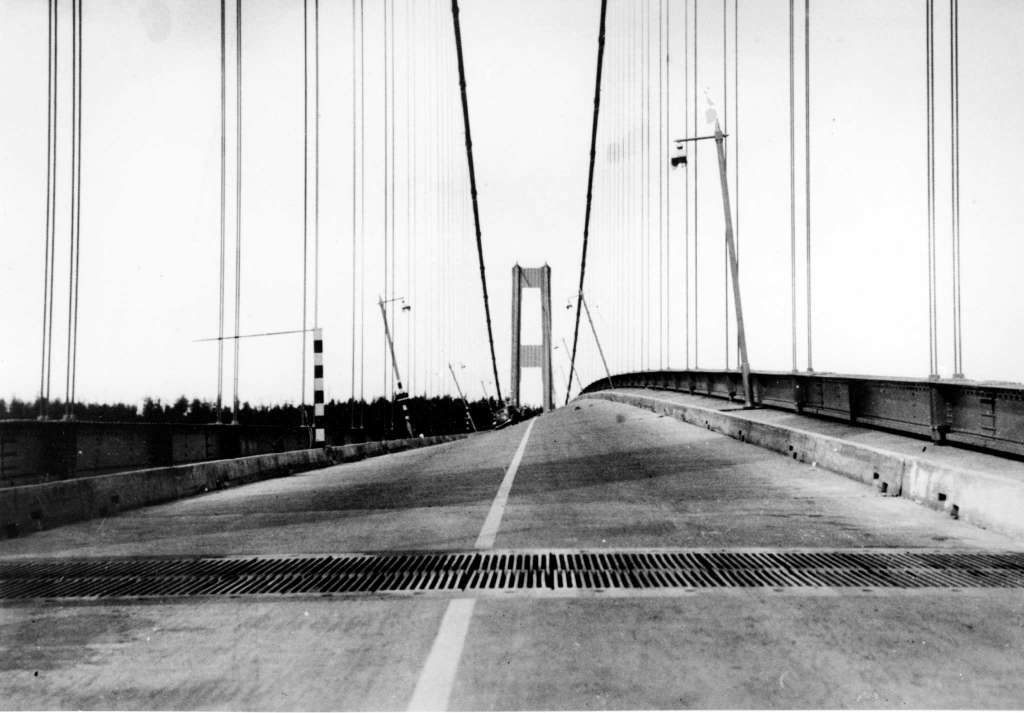
\includegraphics[width=.95\linewidth]{./IntroductionToFSI/tacoma2.jpeg}
  \caption{Tacoma bridge still standing with large deformations}
  \label{fig:test1}
\end{minipage}%
\begin{minipage}{.50\textwidth}
  \centering
  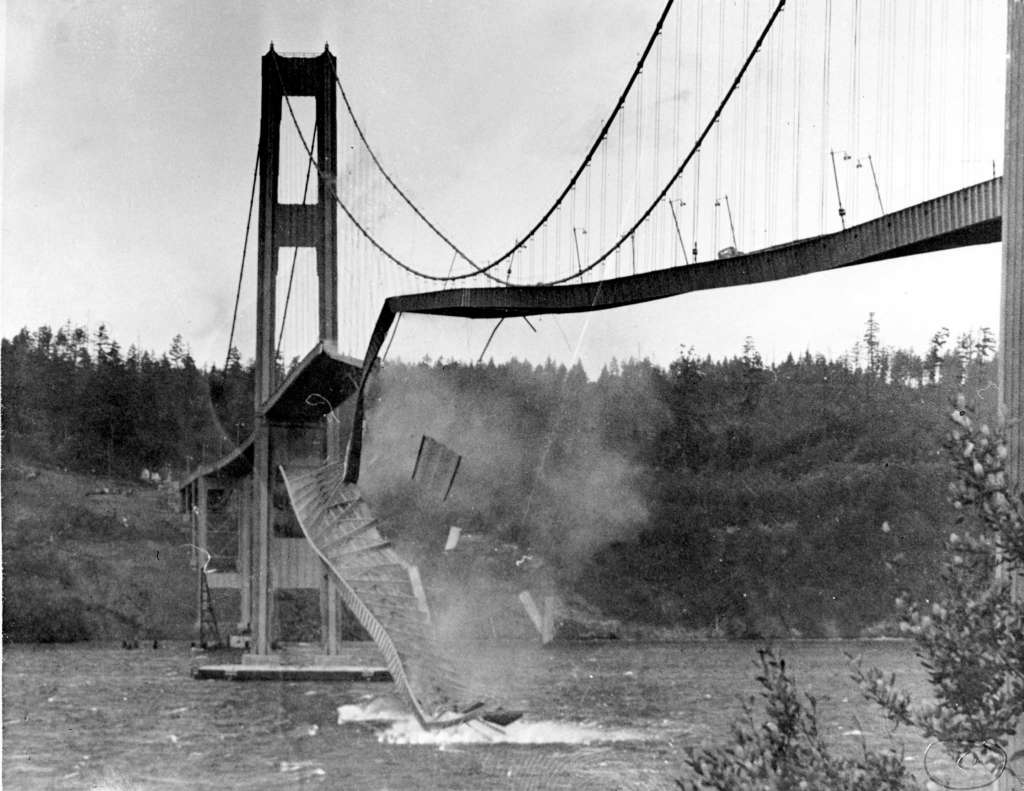
\includegraphics[width=.95\linewidth]{./IntroductionToFSI/tacoma3.jpeg}
  \caption{Tacoma bridge collapsed}
  \label{fig:test2}
\end{minipage}
\end{figure}

Modelling fluid dynamics is called \textit{Computational Fluid Dynamics} (CFD). I would argue the same for FSI. That we call modeling FSI for \textit{Computational Fluid Structure Interaction} (CFSI)
Modeling FSI is used today when constructing for instance windmills. These windmills are usually rigid, hence giving a big difference in density between fluid and structure. The structure will in this case only give rise to small deformations. However modeling FSI in hemodynamics(dynamics of blood flow) deems more challenging. In these cases the densities in fluid and solid are much more similar and usually inducing large deformations. Also in both of these cases the fluid flow tends to transition to turbulence. We can see that these challenges gives the need to have rigid stabile FSI solvers, solvers which can handle large deformations and high fluid velocity. \newline

Tthe main goal of this master thesis is to build a framework to solve the FSI problem, investigating different approaches and schemes. The framework will be validated and verified using the \textit{Method of Manufactured Solutions}, accompanying a wide range of benchmarks.  



\begin{comment}
Fluid-Structure Interaction problem can be observed all around us in nature, from large industrial engineering complexes to the smallest blood vessels in the human body. A large scale example is the collapse of the Tacoma Narrows Bridge that collapsed in 1940 only two months after being opened. The collapse was due to aero-elastic fluttering from strong winds. No human life was lost in the collapse, but a cocker spaniel name Tubby left in a car was not so lucky. The construction of windmills are a second example of the Fluid-Structure Interaction problem. Todays windmills are rigid and hence giving a big difference in density between fluid and structure, $ \rho_s >> \rho_f $. The structure will therefore only give rise to small deformations. However applying FSI to hemodynamics( dynamics of blood flow ) deems more challenging. One FSI hemodynamic problem are inter-cranial aneurysms, which are balloon shaped geometries often occurring where a blood vessel splits into two parts, due to weak vessel walls. Bursting of one of these aneurysms in the skull can have fatale consequences. With fluid and structure densities more equal than the previous example, the structure has an elastic character giving under the right circumstances large deformations. The blood flow also transitions to turbulent flow. This combination gives the need for a rigid stabile solver. Therefore the main goal of this master thesis is to build a framework to solve the FSI problem, investigating different approaches and schemes. The framework will be validated and verified using MMS, companying a wide range of benchmarks.  
\end{comment}

	

\chapter{Continuum mechanics in different frames of reference}
All materials are made up of atoms, and between atoms there is space. The laws that govern these atoms are complex and are very difficult to model. However materials like solids and fluids can be modeled if we assume them to exist as a continuum. This means that we assume that there exist no space inside the materials and they fill completely up the space they occupy. 
We can use mathematics with basic physical laws to model fluids and solids when they are assumed continuous. These laws are generally expressed in two frames of reference, Lagrangian and Eulerian. To exemplify these frameworks we can imagine a river running down a mountain. In the Eulerian framework we are the observer standing still besides the river looking at the flow. We are not interested in each fluid particle but only how the fluid acts as a whole flowing down the river. This approach fits the fluid problem as we can imagine the fluid continuously deforming along the river side. \newline

In the Lagrangian description we have to imagine ourselves on a leaf going down the river with the flow. Looking out as the mountain moves and we stand still compared to the fluid particles. This description fits a solid problem nicely since we are generally interested in where the solid particles are in relation to each other. For instance modeling a beam attached to a wall at one end and a weight at the other end. We can imagine the beam bending and to model this bending we need to where all the particles are compared to each other. The more force that is applied the more the particles move in relation to eachother. \newline

In this chapter I will introduce both of these frameworks and the equations which are needed to model Fluid and Structure separately. I start with the Lagrangian description, by providing a short introduction to Lagrangian physics for the sake of completeness. Then introduce the solid and fluid equations. For a more detailed look on Lagrangian physics and the solid equation see \cite{Holzapfel2000}.


\section{Conservation of mass and momentum for solid matter}
With matter assumed continuous, fundamental physical laws like conservation of mass and conservation of momentum can be applied to derive a differential equation describing the motions of a solid. Information about the particular material of a solid is added through constitutive relations.
The differential solid equation will be stated in the Lagrangian reference system \cite{Holzapfel2000}, in the solid domain $\mathcal{S}$ as:
\begin{equation}\label{eq:Solid}
\rho_s \frac{\partial \bold{d}^2}{\partial t^2} = \nabla \cdot ( P ) + \rho_s f  \hspace{4mm} in \hspace{2mm} \mathcal{S}
\end{equation}
written in terms of the deformation $\bold{d}$, of the solid.
P is the first Piola-Kirchhoff stress tensor, its derivation is included in the appendix A1 for the sake of completeness.
Body forces are denoted as $f$, and are forces that originate outside the body and act on the mass of the body e.g. gravitational force. $\rho_s$ is the solid density, and $\frac{\partial}{\partial t^2}$ is the second time derivative. 

\begin{comment}
\subsection*{Locking}
The problem og shear locking can happen FEM computations with certain elements. 
[mek4250 Kent] - Locking occurs if  $ \lambda >> \nu $ that is, the material is nearly incompressible. The reason is that all the elements discussed in this course are poor at approximating the divergence. Locking refers to the case where the displacement is to small because the divergence term essentially lock the displacement. It is a numerical artifact not a physical feature. [Verbatum]
\end{comment}

\section{Fluid equations}
The Navier-Stokes equations are derived using principles of mass and momentum conservation. These equations describes the velocity and pressure in a given fluid continuum. They are here written in the time domain $\mathcal{F}$:
\begin{align}
\label{eq:NS}
\rho\frac{\partial u}{\partial t} + \rho u \cdot \nabla u &= \nabla \cdot \sigma_f + f \\
\nabla \cdot u &= 0
\end{align}
where $u$ is the fluid velocity, $p$ is the fluid pressure$, \rho$ stands for constant density, f is body force and $ \sigma_f = \mu_f (\nabla u + \nabla u^T)  - pI$ \\
We will only compute incompressible fluids. \\
There does not yet exist an analytical solutions to the N-S equations, only simplified problems can be solved \cite{White2000}. But this does not stop us from discretizing and solving them numerically. \\
Before these equations can be solved we need to impose boundary conditions.
\subsection*{Boundary conditions}
On the Dirichlet boundary $ \partial \mathcal{F}_D$ we impose a given value. This can be initial conditions or set to zero as on walls with "no slip" condition. These conditions needs to be defined for both $u$ and $p$
$$  u = u_0 \text{   on   } \partial \mathcal{F}_D  $$
$$  p = p_0 \text{   on   } \partial \mathcal{F}_D  $$
The forces on the boundaries need to equal an eventual external force $ \bold{f}$
$$ \sigma \cdot \bold{n} = f \text{   on   } \partial \mathcal{F}_N    $$









\begin{comment}
Let $\Omega \in \mathbb{R}^d $ for $d \in \{1,2\}$, be a bounded domain with boundary $ \partial \Omega$. The domain is made up of of two sub domains $ \mathcal{F} $ for the fluid domain, and $\mathcal{S}$ for the solid. The interface between the domains are denoted by $ \Sigma = \mathcal{F} \cap \mathcal{S} $. The reference or initial is denoted by $ \hat{\Sigma} = \hat{\mathcal{F}} \cap \hat{\mathcal{S}}  $ 
\end{comment}



\chapter{Fluid Structure Interaction Problem}
In this chapter I will introduce the full FSI problem. With all the equations, conditions, and discretizations needed to to build a Fluid Structure Interaction solver. \newline

When we compute FSI problems the computing domain is split into three parts, fluid, structure and interface. Fluid and structure domains are as we know separated, and different constitutive equations are solved in each domain. The place in which fluid and structure meet is what we call the interface. The manner in which we treat the interface gives the two main methods for solving FSI problems \cite{Liu2014}. The first method is called fully Eulerian. In fully Eulerian both the fluid and structure equations are solved in an Eulerian description. Here the interface is tracked across a still standing domain \cite{Valkov2015}. The fully Eulerian description is suited for fluid problems but is problematic for structure problems and certainly FSI where tracking of the interface across the domain is a difficult task. \newline

The second approach is the \textit{Arbitrary Lagrangian Eulerian}
The ALE method entails formulating the fluid equations in a type of Eulerian framework and the solid in a Lagrangian framework. The entire domain itself moves with the structural displacements and the fluid moves through these points. In the ALE framework we get best of both world, in that fluid and solid are described in their natural states. The structure equation will remain as previously stated \eqref{eq:Solid}, and we will need to change the fluid equations to take into account the moving domain changing the fluid velocity. Dealing with the movement of the domain is done in two ways. One way is to move the domain itself in relation to the structural displacements, and use this new domain to calculate the equations every time.
Moving the domain gives advantages as we can explicitly represent the fluid-structure interface, and the equations are stated in a more familiar manner. But problems arise when there are large deformations in the solid giving large deformations into the fluid domain. Moving the mesh with large deformation can be a challenge in that the domain can overlap causing singularities. \newline

\textbf{In this thesis the ALE approach is used from a reference frame.}
Meaning we solve the equations on a initial, stress free domain, and use a series of mappings to account for the movements of the domain. The equations are mapped to the current domain, that is where the domain has moved to in the present time. It is the displacements in the in the domain that determines the mappings between frames of reference. The displacements in the solid and the interface are extrapolated into the fluid mesh. \newline

From a technical point of view, both moving the mesh and using a reference frame are equivalent \cite{Richter2016}. Since the reference frame method does not need a function to move the mesh between each time iteration, it can be less time consuming. The interface is also located in the same position, making the interface easy to track. \newline

There are generally two types of schemes used when simulating FSI. The first is the partitioned approach where fluid and structure are solved sequentially.  This approach is appealing in that we have a wealth of knowledge and techniques on how to solve each of these kinds of problems in an efficient manner. The difficulty however is dealing with the interface. As we know there are kinematic and dynamic conditions needed in FSI, and the coupling of these conditions is where the problems arise. So called explicit coupled schemes are known to be unconditionally unstable for standard Dirichlet-Neumann strategies when there is a large amount of added-mass in the system \cite{Fernandez2015}, \cite{VanBrummelen2009}. There are however, schemes which offer added-mass free stability with explicit coupling, where the interface is treated through a Robin-Neumann coupling. First for a coupling with a thin walled structure \cite{Fernandez2013} and later with an extension to thick wall \cite{Fernandez2015}. These schemes are rather complex and uses a number of techniques that are out of the scope of this thesis. ( This may be in more detail in a later chapter (discussion and further work.) ) \newline

The other approach is called monolithic. In the monolithic approach all of the equations are solved at once. This approach has the advantage of offering numerical stability for problems with strong added-mass effects \cite{Liu2014}, and are fully coupled. The disadvantage over the partitioned approach is that we loose flexibility when solving many equations simultaneously, and the problems can quickly become large and computationally costly. \newline

I will start by introducing the mappings needed to change between current and reference domain, this follows the notation and ideas from \cite{Richter2016}:

\section{Mapping between different frames of reference}
\begin{figure}[H]
\label{pic:FSI_mapping}
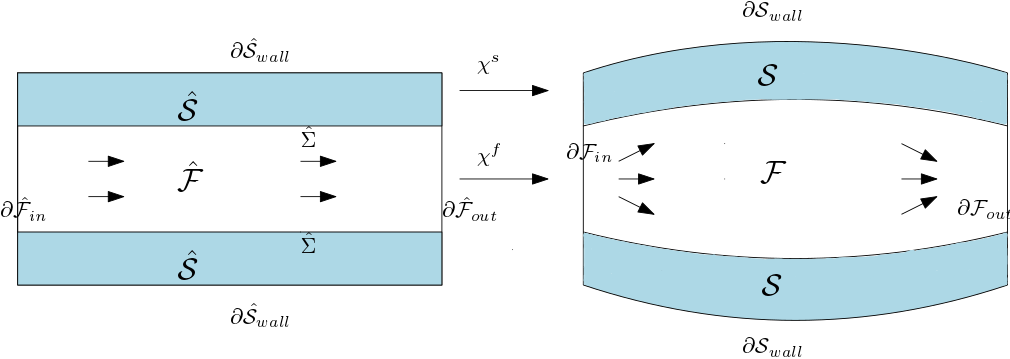
\includegraphics[scale=0.45]{./FSI_ALE_formulation/FSI_mapping.png}
\caption{Mapping of domain from reference to current}
\end{figure}

Let $\hat{\mathcal{V}}$ be a reference volume and $\mathcal{V}(t)$ be the current time volume. Then using \eqref{eq:deformation_gradient} and \eqref{eq:J} we define a mapping between the volumes from the current to reference configurations:

\begin{equation}
 \int_{\mathcal{V}(t)} 1  dx = \int_{\hat{\mathcal{V}}} J dx  
\end{equation}

The gradients acting on a vector $ \bold{u} $ will also be mapped between current and reference configurations:

\begin{equation}
\int_{\mathcal{V}(t)} \nabla \bold{u}   dx = \int_{\hat{\mathcal{V}}} J  \nabla \bold{u}F^{-1} dx  
\end{equation}

Same for the divergence of a vector $ \bold{u}$:

\begin{equation}
\int_{\mathcal{V}(t)} \nabla \cdot \bold{u}   dx = \int_{\hat{\mathcal{V}}} \nabla \cdot( J  F^{-1} \bold{u}) dx  
\end{equation}

\section{Governing equations for Fluid Structure Interaction}

We will formulate the equations in the Eulerian, Lagrangian and the ALE description. We start by briefly talking about time derivatives in the different configurations. In the Lagrangian setting the total and partial derivatives are the same \cite{Wick2011}:

\subsection{Derivatives in different frameworks}
\begin{equation}
D_t f(x,t) = \partial_t f(x,t) 
\end{equation}

in the Eulerian framework we have the following relation between total and partial derivatives:

\begin{equation}
D_t f(x,t) = \bold{u}\cdot \nabla{f} + \partial_t f(x,t)
\end{equation}

whilst in the ALE framework we extend this concept to take into account the motion of the domain:

\begin{equation}
D_t f(x,t) = \bold{w} \cdot\nabla{f} + \partial_t f(x,t)
\end{equation}

Here we can see that for the Lagrangian framework $ \bold{w}$ is zero and for Eulerian $\bold{w} = \bold{u}$.

\subsection{Solid equation}
We express the solid balance laws in the Lagrangian formulation from the initial configuration

\begin{equation}
\rho_s \frac{\partial \bold{u}}{\partial t} = \nabla \cdot (P) + \rho_s f \hspace{4mm}in\hspace{4mm} \hat{\mathcal{S}} 
\end{equation}
written in terms of the solid velocity $\bold{u} = \bold{u_s} = \frac{\partial \bold{d}}{\partial t}$.

\subsection{Fluid equations}


The fluid domain is moving, and therefore we need to redefine the velocity in the convective term in \eqref{eq:NS} to account for the moving domain 
\begin{equation}
\bold{u} \cdot \nabla \bold{u} \rightarrow (\bold{u}-\frac{\partial \bold{d}_f}{\partial t}) \cdot \nabla \bold{u}  
\end{equation}
where $d_f$ is the deformation in the fluid domain. We see that $\bold{w}$ is written as $\frac{\partial \bold{d}}{\partial t}$ . Now the actual fluid convection will be $\bold{u}-\frac{\partial \bold{d}}{\partial t} \nabla \bold{u}$ 

The fluid equations are denoted from the initial configuration using the aforementioned mappings:

\begin{align}
\int_{\mathcal{V}(t)} \rho_f \frac{\partial \bold{u}}{\partial t} dx & = \int_{\hat{\mathcal{V}}}  \rho_f J \frac{\partial \bold{u}}{\partial t} dx \\
\int_{\mathcal{V}(t)} \nabla \bold{u} (\bold{u}-\frac{\partial d}{\partial t}) dx  &= \int_{\hat{\mathcal{V}}} ((\nabla \bold{u})F^{-1}(\bold{u}-\frac{\partial d}{\partial t}) dx  \\
\int_{\mathcal{V}(t)} \nabla \cdot \bold{u} dx  &=\int_{\hat{\mathcal{V}}}  \nabla \cdot (J F^{-1} \bold{u}  ) dx \\
\int_{\mathcal{V}(t)} \nabla \cdot \sigma_f dx &= \int_{\hat{\mathcal{V}}} \nabla \cdot( J F^{-1} \hat{\sigma_f} )     dx \\
\hat{\sigma_f} &= -pI + \mu ( \nabla \bold{u} F^{-1} + F^{-T} \bold{u}^{T}  ) 
\end{align}

Assembling all these terms together with \eqref{eq:NS} gives the fluid equations from a reference frame:

\begin{align}
\label{eq:NS_mapped}
\rho_f J \big( \frac{\partial \bold{u}}{\partial t} dx + (\nabla \bold{u})F^{-1}(\bold{u}-\frac{\partial \bold{d}}{\partial t}) \big) &= \nabla \cdot( J F^{-1} \hat{\sigma_f} ) + J \rho_f f \\
\nabla \cdot (J F^{-1} \bold{u} ) &= 0
\end{align} 

\section{Mesh motion techniques} \label{sec:meshmotion}
Using the ALE method the deformations from the structure through the interface is extrapolated to the fluid domain. The choice of mesh motion technique is important for the overall FSI problem to be calculated \cite{Wick2011a}. When large deformations occur, we need a good lifting operator to uphold the integrity of the computing domain. A poor choice will make the mesh overlap and singularities may occur. 
When extrapolating deformation from the solid to the fluid domain, the fluid domain itself acts as a structure, deforming according to the deformations from the structure domain.
I will in this section present different mesh motion techniques, that act differently on the computational domain. In \ref{sec:mesh_motion} the techniques will be tested and investigated.

\subsection{Harmonic extension}
For small to moderate deformations we can use a harmonic extension to lift the deformations. The harmonic extenstion uses the Laplace equation, transporting the deformations from the solid into the fluid domain. A variable $\alpha_u > 0$ can be multiplied to the Laplace equation, to control the amount of lifting of deformations to the fluid domain.

\begin{align}
 - \alpha_u \nabla^2 \bold{d} =& 0\hspace{4mm} in \hspace{2mm} \hat{\mathcal{F}}\\
  \hspace{4mm} \bold{d} =& 0 \hspace{4mm } on \hspace{2mm }  \partial \hat{\mathcal{F}} / \hat{\Sigma} \\
  \bold{d}_f =& \bold{d}_s \hspace{4mm } on \hspace{2mm } \hat{\Sigma} 
\end{align}

When using the harmonic lifting operator the variable $\alpha_u$ is very important when calculating moderate deformations. For small deformations a constant can be used for $\alpha_u$. But for larger deformations we need to be a bit more clever. A good strategy for choosing $\alpha_u$ is proposed by Wick in \cite{Wick2011a}, and further discussed in \cite{Stein2003} and \cite{MM2016}. Which is an alpha that gets bigger when closer to the interface. 
\begin{equation}
\alpha_u = \frac{1}{x^q}
\end{equation}
where $x^q$ is the distance from the interface. If $q=0$ the laplacian i recovered. When the distance becomes larger, $\alpha_u$ gets smaller, and vice versa. 
Defining $\alpha_u$ in this manner is a smart choice since it upholds the cell structure closer to the interface where most of the cell distortion appears. 

\begin{comment}
\subsection{Linear elastic extension}
Since the fluid domain acts as structure we can use a linear elastic equation to lift the deformations from the solid into the fluid domain. The linear elastic equation is best known from computing solid problems \cite{Wick2011a}.  The model is as follows:

\begin{align}
-\nabla \cdot \sigma_{mesh} &= 0 \hspace{4mm} in \hspace{2mm} \hat{\mathcal{F}}\\
\hspace{4mm} d &= 0 \hspace{4mm } on \hspace{2mm }  \partial \hat{\mathcal{F}} / \hat{\Sigma} \\
\sigma_{mesh} &= \alpha_\lambda (tr\epsilon)I + 2\alpha_\mu \epsilon 
\end{align}
where $\epsilon = \frac{1}{2}(\nabla d + (\nabla d)^T)$. $\epsilon$ is the linearized version of the strain tensor \eqref{eq:StrainTensor}. The parameters $\alpha_\lambda$ and $\alpha_\mu$ are chosen to uphold domain quality. This is done by computing the parameters $\alpha_\lambda$ and $\alpha_\mu$ from Youngs modulus and poisson ration. 

\end{comment}

\subsection{Biharmonic extension} 
The last extension is the biharmonic extension. The biharmonic extension provides more freedom than the harmonic and linear elastic in choosing boundary conditions and choice of parameter $\alpha_u > 0$. This is because the biharmonic extension, extends the deformation in a manner that upholds the integrity of the cells even in large deformations, even with $\alpha_u$ as a constant. In its simplest form it is written as:

\begin{equation}
- \alpha_u \nabla^4 d = 0 \hspace{4mm}  in \hspace{2mm} \hat{\mathcal{F}}\\
\end{equation}

The biharmonic extension is calculated with a mixed formulation where we introduce a new function $\omega$ (not to be confused with the deformation velocity), this function is added to the system so that we solve for 4 functions:

\begin{equation}
\omega = \alpha_u \nabla^2 \bold{d} \hspace{4mm} and \hspace{4mm} - \alpha_u \nabla^2 \omega = 0 \hspace{2mm}   in \hspace{2mm} \hat{\mathcal{F}}
\end{equation}
with the two types of boundary conditions. The first being:
\begin{align}
\bold{d} = \partial_n \bold{d} =& 0 \hspace{4mm} on \hspace{2mm} \partial \hat{\mathcal{F}} \hspace{2mm} \textbackslash \hspace{2mm} \hat{\Sigma}\\
\bold{d}_f =& \bold{d}_s \hspace{4mm } on \hspace{2mm } \hat{\Sigma} 
\end{align}

The second imposes conditions on $\bold{d}$ and $\omega$, and are written in terms of single component functions $d^{(1)},d^{(2)}$ and $\omega^{(1)}, \omega^{(2)}$	
\begin{align}
\bold{d}^{(1)} =& \partial_n d^{(1)} = 0 , and \hspace{4mm}   \omega^{(1)} = \partial_n \omega^{(1)} = 0    \hspace{4mm} on \hspace{2mm} \partial \hat{\mathcal{F}}_{in,out} \\
\bold{d}^{(2)} =& \partial_n d^{(2)} = 0 , and \hspace{4mm}   \omega^{(2)} = \partial_n \omega^{(2)} = 0    \hspace{4mm} on \hspace{2mm} \partial \hat{\mathcal{F}}_{walls} \\
\end{align}

Since the biharmonic extension is of fourth order character it will have a higher computational cost \cite{Richter2016} than the harmonic or linear elastic. 


\section{Coupled Fluid Structure Interface conditions}
In figure \ref{pic:FSI_mapping} we see a typical Fluid Structure Interaction. The fluid is surrounded by elastic walls, like a blood vessel. The inflow at $\partial \hat{\mathcal{F}}_{in}$, a change in pressure, or a motion of the solid determines the flow of the fluid.
The fluid`s stress on the walls causes deformation in the solid domain and vice versa. The interface is where these energies are transferred and we therefore need conditions on the interface. \newline

Let $\Omega \in \hat{\mathcal{S}} \cup \hat{\mathcal{F}} $ be a global domain that is made up of the fluid, structure, and the interface. We define a global velocity function $u$ that describes the fluid velocity in the fluid domain and the structure velocity in the structure domain. Using a global velocity makes the velocity continuous across the entire domain. Let interface be $ \hat{\Sigma} \in \hat{\mathcal{S}} \cap \hat{\mathcal{F}}  $.\newline 
The three interface comes from simple physical properties and consist of \cite{Richter2016}:

\begin{itemize}
\item \textit{Kinematic condition}: $\bold{u}_f = \bold{u}_s  \hspace{2mm} on \hspace{2mm} \hat{\Sigma}$. The fluid and structure velocities are equal on the interface. Meaning the fluid moves with the interface at all times. \\
Since we use a global function for $\bold{u}$ in both fluid and structure domains, this condition is upheld.\\ 
The fluid and solid velocities are usually in different coordinate systems, the solid velocity is then not available in Eulerian Coordinates. We instead link fluid velocity at the interface by using the fact that $\bold{u}_s = \frac{\partial d}{\partial t}$. Setting $\bold{u}_f = \frac{\partial d}{\partial t}$ at the interface.

\item \textit{Dynamic condition}: $  \sigma_f n_f = \sigma_s n_s \hspace{2mm} on  \hspace{2mm}\hat{\Sigma}   $. \\
	This relates to Newtons third law of action and reaction. The forces on the interface area, here written as the normal stresses are balanced on the interface. These will be written in a Lagrangian formulation: \\
	$J\sigma_f F^{-T} n_f = P n_s \hspace{2mm} on  \hspace{2mm}\hat{\Sigma} $. \\
	The dynamic condition is a Neumann condition that belongs to both subproblems.
	
\item \textit{Geometrical condition}: This condition says that the fluid and structure domains do not overlap, but rather that elements connect so the functions needing to transfer force are continuos across the entire domain.
\end{itemize}



\begin{comment}
We start by stating the entire FSI ALE problem in a monolithic framework using the mapped approach: 

Find $\bold{u} \in \hat{\mathcal{F}} , p \in \hat{\mathcal{F}} \text{  and  } d \in \hat{\mathcal{S}} \text{  such that}:$ 
\begin{align}
\rho_f J \big( \frac{\partial u}{\partial t} + (\nabla \bold{u} )F^{-1}(\bold{u} -\frac{\partial d}{\partial t})\big)  + \nabla \cdot( J \hat{\sigma_f} F^{-T})  &= 0 \hspace{8mm}\text{on  } \hat{\mathcal{F}} \\
\nabla \cdot (J \bold{u}  F^{-T})\big) &= 0 \hspace{8mm} \text{on  } \hat{\mathcal{F}}   \\
\rho_s \frac{\partial \bold{u} }{\partial t} + \nabla \cdot F S_s,&=0 \hspace{8mm} \text{on  } \hat{\mathcal{S}}\\
\nabla^2 d &= 0 \hspace{8mm} \text{on  } \hat{\mathcal{F}}\\
\bold{u} - \frac{\partial d}{\partial t}  &= 0 \hspace{8mm} \text{on  } \hat{\mathcal{S}}\\
J\sigma_f F^{-T} n_f &= \sigma_s  n_s \hspace{3mm} \text{on  } \hat{\Sigma}
\end{align}
\end{comment}

\section{Discretization of monolithic FSI equations}\label{Discretization}
After introducing all the equations and boundary conditions needed to solve a FSI problem. We are ready to discretize the equations into one monolithic scheme. The equations will be discretized and solved using finite difference and finite element methods. I will introduce a so called $\theta$-scheme which will make it easy to implement different schemes, by choosing a value for $\theta$.
I will briefly introduce the spaces needed to discretize, following the ideas and notations of \cite{Wick2011}:

\subsubsection{Spaces}
Let $ X \in \mathbb{R}^d , d \in\{ 1,2  \} $ be a time dependent domain we define:

\begin{equation}
\hat{V}_X := H^1(X), \hspace{6mm}  \hat{V}^1_X := H^1_0(X) 
\end{equation}

$ H^1 $ indicating a Hilbert space and

\begin{equation}
\hat{L}_X := L^2(X), \hspace{6mm} \hat{L}^0_X := L^2(X) / \mathbb{R}
\end{equation}

$L^2$ indicating a standard Lebesque space.

The trial and test spaces for the velocity variable in the fluid domain,

\begin{equation}
\hat{V}^0_{f,u} := \{ \hat{u} \in H^1_0(\mathcal{F}) : \hat{u}_f = \hat{u}_s \hspace{2mm} on \hspace{2mm} \hat{\Sigma}  \}
\end{equation}

and the same for the artificial displacement in the moving fluid domain:

\begin{equation}
\hat{V}^0_{f,d} := \{ \hat{d} \in H^1_0(\mathcal{F}) : \hat{d}_f = \hat{d}_s \hspace{2mm} on \hspace{2mm} \hat{\Sigma}  \}
\end{equation}
\begin{equation}
\hat{V}^0_{f,d} := \{ \hat{d} \in H^1_0(\mathcal{F}) : \hat{\psi_f} = \hat{\psi_s} \hspace{2mm} on \hspace{2mm} \hat{\Sigma}  \}
\end{equation}

Now that the spaces have been defined we are ready to discretize. The temporal discretization is done using finite difference schemes and the spatial is treated with the finite element method. I will employ a $\theta-$ scheme that will enables us to easily switch between schemes.

\subsubsection{Discretization}

In the domain $\Omega$ and time interval [0,T]:

Find $ U = \{\bold{u}, d, p\} \in \hat{X}^0_D $ where $ \hat{X}^0_D := \{ \bold{u}^D_f + \hat{V}^0_{f,\bold{u}} \} \times \hat{L}_f \times \{ d_f^D + \hat{V}^0_{f,\hat{f}} \} \times \{ d_f^D + \hat{V}^0_{f,\hat{f}} \} \times \hat{L}^0_f \times \hat{L}^0_s  $ such that:

\begin{equation}
\int_0^T A(U)(\Psi) dt = \int_0^T \hat{F}(\Psi) dt \hspace{4mm} \forall  \Psi \in \hat{X}
\end{equation}

where $ \Psi = \{\phi, \psi, \gamma \} $% \hat{\psi}^\bold{u}_f, \hat{\psi}^\bold{u}_s, \hat{\psi}^d_f, \hat{\psi}^d_s, \hat{\psi}^p_f,\hat{\psi}^p_f  \}$ and

 $\hat{X} = \hat{V}^0_{f,\bold{u}} \times \hat{L}_f \times \hat{V}^0_{f,d,\hat{\Sigma}} \times \hat{V}_s^0 \times \hat{L}_f^0 \times \hat{L}_s^0  $


I first introduce the scheme using, for simplicity, the harmonic mesh motion. Let $\bold{u}$ be a global function in the entire domain instead of $\bold{u}_f$ in the fluid and $\bold{u}_s$ in the solid. Same for the test functions. This is done for ease of reading and also for the ease of implementation later.

\textbf{The full monolithic FSI variational form reads}:
\begin{align}
A(U)&= (J \rho_f \partial_t \bold{u} , \phi ) - (J (\nabla u)F^{-1}(\bold{u} - \partial_t d) , \phi )_{\mathcal{\hat{F}}}  \\
       &+ ( J \sigma_{f} F^{-T} , \nabla \phi )_{\mathcal{\hat{F}}} \\
       &+ (\rho_s \partial_t \bold{u} , \phi)_{\mathcal{\hat{S}}}   + \big(F S_s, \nabla \phi \big)_{\mathcal{\hat{S}}} \\
       &+ ( \alpha_u \nabla \bold{u}, \nabla \psi)_{\mathcal{\hat{F}}} + (\nabla \cdot (J F^{-1} \bold{u}),\gamma )_{\mathcal{\hat{F}}} \\
       \label{eq:condition}
       &+ \delta\big((\partial_t \bold{d} , \psi)_{\mathcal{\hat{S}}}  - ( \bold{u} , \psi )_{\mathcal{\hat{S}}}\big) \\ 
       &+  \big( J \sigma_{f,p} F^{-T}, \nabla \phi  \big) 	 		
\end{align}

The condition \eqref{eq:condition} , is weighted with a $\delta$ value. This is a critical detail for the program (detailed later) to run. The only two places where we use the test function $\psi$ is on this condition and the lifting operator. The weighting says in a weak manner that this condition is important for the overall program. \newline

I will here formulate the \textit{One step-$\theta$ scheme} from \cite{Wick2011}. This $\theta$ scheme has the advantage of easily being changed from the backward (implicit), forward(excplicit) or Crank-Nicholson (implicit) scheme. The Crank-Nicholson scheme is of second order, but suffers from instabilities in this monolithic scheme \cite{Wick2011}. A remedy for these instabilities is to chose a Crank-Nicholson scheme that is shifted towards the implicit side. How this is done will become evident once the scheme is defined.

We define the variational form by dividing into four categories, this may seem strenuous at first but the need for it will become evident when implementing the $\theta$-scheme. The four divided categories consists of: a time term, implicit, pressure and the rest (stress, convection):

\begin{align}
A_T(U) &= (J \rho_f \partial_t \bold{u} , \phi ) - (J (\nabla u)F^{-1}(\partial_t \bold{d}) , \phi )_{\mathcal{\hat{F}}} \\
	    & + (\rho_s \partial_t \bold{u} , \phi)_{\mathcal{\hat{S}}} + (\partial_t \bold{d} , \psi)_{\mathcal{\hat{S}}}  \\
A_I(U) &= ( \alpha_u \nabla \bold{u}, \nabla \psi)_{\mathcal{\hat{F}}} + (\nabla \cdot (J F^{-1} \bold{u}), \gamma)_{\mathcal{\hat{F}}} \\
A_E(U) &= (J (\nabla u)F^{-1} \bold{u} , \phi )_{\mathcal{\hat{F}}} + ( J \sigma_{f,u} F^{-T} , \nabla \phi )_{\mathcal{\hat{F}}} \\
	    & + \big(F S_s, \nabla \phi \big)_{\mathcal{\hat{S}}} - ( \bold{u} , \psi )_{\mathcal{\hat{S}}} \\
A_P(U) &= \big( J \sigma_{f,p} F^{-T}, \nabla \phi  \big)  	 		
\end{align}

Notice that the stress tensors have been split into a velocity and pressure part. 
\begin{align}
\sigma_{f,u} &= \mu ( \nabla u F^{-1} + F^{-T} \nabla u) \\
\sigma_{f,p} &= -p I
\end{align}

For the time group, discretization is done in the following way:
\begin{align}
A_T(U^{n,k}) \approx & \frac{1}{k} \big( \rho_f J^{n,\theta} (\bold{u}^n - \bold{u}^{n-1}) , \phi  \big)_{\mathcal{\hat{F}}} - \frac{1}{k} \big( \rho_f (\nabla u ) (\bold{d}^n - \bold{d}^{n-1}) , \phi \big)_{\mathcal{\hat{F}}} \\
+ & \frac{1}{k} \big( \rho_s  (\bold{u}^n - \bold{u}^{n-1}) , \phi  \big)_{\mathcal{\hat{S}}} +  \frac{1}{k} \big( (\bold{d}^n - \bold{d}^{n-1}) , \psi  \big)_{\mathcal{\hat{S}}}
\end{align}
And the Jacobian is written with superscript $\theta$ as:

\begin{equation}
J^{n, \theta} = \theta J^n + (1-\theta)J^{n-1}
\end{equation}

We can now introduce the \textit{One step-$\theta$ scheme}: 
Find $U^n = \{\bold{u}^n , \bold{d}^n, p^n \}$

\begin{align}
& A_T(U^{n,k}) + \theta A_E(U^{n}) + A_P(U^{n}) + A_I(U^{n}) = \\
& - (1-\theta) A_E(U^{n-1}) + \theta \hat{f}^n + (1-\theta) \hat{f}^{n-1}  
\end{align}

We notice that the scheme is selected by the choice of $\theta $. By choosing $ \theta = 1$ we get the back Euler scheme, for $ \theta = \frac{1}{2}$ we get the Crank-Nicholson scheme and for the shifted Crank-Nicholson we set $ \theta = \frac{1}{2} + k$, effectively shifting the scheme towards the implicit side. $\hat{f}$ is the body forces which will be ignored in this thesis. The shifting toward the implicit side is important for long term stability for certain time step values \cite{Wick2011}. The shifting will be investigated in the next chapter.







\subsection{Spaces and Elements}
The velocity and pressure copling in the fluid domain must satisfy the inf-sup condition. If not stabilization has to added. We here need to define some spaces that will have these desired properties.
We denote $u_h \in V_h$ and $ d_h \in W_h $, here the finite element pair og pressure and velocity mush satisfy the inf-sup condition given in ALE coordinates:
$$   \inf_{\substack{p_h \in L_{h,f}}}  \sup_{\substack{v_h \in V_{h,f}}} \frac{ (p_h, div(J_f F_f^{-1} u_h))_{\mathcal{F}} }{ \|\|J^{\frac{1}{2}} p_h  \|\|_{\mathcal{F}} \|\|  J^{\frac{1}{2}}_{f} \nabla u_h F_f^{-T} \|\|_{\mathcal{F}}  } \geq \hat{\Sigma}     $$
A good choice of spaces will be P2-P2-P1 for velocity, displacement and fluid pressure respectively. 









%\begin{comment}
\lstdefinelanguage{Python}{
 keywords={typeof, null, catch, switch, in, int, str, float, self},
 ndkeywords={boolean, throw, import},
 ndkeywords={return, class, if ,elif, endif, while, do, else, True, False , catch, def},
 ndkeywordstyle=\color{blue}\bfseries,
 identifierstyle=\color{black},
 sensitive=false,
 comment=[l]{\#},
 morecomment=[s]{/*}{*/},
 commentstyle=\color{purple}\ttfamily,
 stringstyle=\color{red}\ttfamily,
 backgroundcolor = \color{lightgray}
}
\end{comment}


\chapter{Implementation of Fluid Structure Interaction in FEniCS}
This Chapter shows the implementation of the FSI code in FEniCS \cite{FENICS}. FEniCS is platform used to solve partial differential equations. Code is written in python and FEniCS makes it easy to run efficient finite element code. \newline

The complete code consist of many hundreds of lines of code, and therefore only the most essential parts are covered. The code that has been added is added so that a reader with a minimal skill set in scientific computing and basic knowledge of the finite element method could implement a version of the code.



\section{Mappings}
The deformation gradient and the Jacobian is made using python functions. The deformation gradient python function takes in the deformation and returns the deformation gradient. Identity in FEniCS is a function that makes the identity matrix, with the size determined by a input value. The identity takes the length of the deformation function which for 2D cases is 2. grad is a built in FEniCS function that takes a vectorfunction and take the gradient.
\begin{python}\caption{Fenics code of deformation gradient and Jacobian}
def F_(d): """inputs deformation """
	return (Identity(len(d)) + grad(d))  """Returns the deformation gradient"""

def J_(d):
	return det(F_(d))
\end{python}


\section{Variational form}

The variational form can be written directly into FEniCS. A big advantage in FEniCS is that one can write all the forms and add them together to make the full variational form.
The vector functions and functions such as the displacement, velocity, and pressure, are written with a script n meaning at which time the function is valued. 
\begin{python}\caption{Deformation, velocity and pressure function described at three different timesteps }
d_["n"]  """deformation in the current timestep """
u_["n-1"] """velocity in the last timestep """
p_["n-2"] """pressure in the second last timestep """
\end{python}

theta is the value $\theta$ that determines the scheme.
k is the timestep $\Delta t$\\
$F_fluid_linear$ is the linear part of the variational form, and $F_fluid_nonlinear$ is the nonlinear part. Each part is assembled later when using newtonsmethod. 

Constant is a function in FEniCS that represents a constant value unknown at compile-time. Its value can be changed without the need to re-compilation of C++ code, which FEniCS utilizes.
$sigma_f$ and $sigma_f $ is the velocity and pressure parts of the fluid stress tensor.
grad and div are built-in functions in FEniCS that computes the gradient and divergence and given vector.
$dx_f$ denotes the fluid domain. 
$inv()$ is a built-in function in FEniCS outputs the inverse of the given matrix. 
psi, phi and gamma are the test functions.

\begin{python}
J_theta = theta*J_(d_["n"]) + (1 - theta)*J_(d_["n-1"]) 

F_fluid_linear = rho_f/k*inner(J_theta*(v_["n"] - v_["n-1"]), psi)*dx_f

F_fluid_nonlinear =  Constant(theta)*rho_f*\
inner(J_(d_["n"])*grad(v_["n"])*inv(F_(d_["n"]))*v_["n"], psi)*dx_f

F_fluid_nonlinear += inner(J_(d_["n"])*sigma_f_p(p_["n"], d_["n"])*\
inv(F_(d_["n"])).T, grad(psi))*dx_f

F_fluid_nonlinear += Constant(theta)*inner(J_(d_["n"])\
*sigma_f_u(v_["n"], d_["n"], mu_f)*inv(F_(d_["n"])).T, grad(psi))*dx_f

F_fluid_nonlinear += Constant(1 - theta)*inner(J_(d_["n-1"])*\
sigma_f_u(v_["n-1"], d_["n-1"], mu_f)*inv(F_(d_["n-1"])).T, grad(psi))*dx_f

F_fluid_nonlinear += \
inner(div(J_(d_["n"])*inv(F_(d_["n"]))*v_["n"]), gamma)*dx_f

F_fluid_nonlinear += Constant(1 - theta)*rho_f*\
inner(J_(d_["n-1"])*grad(v_["n-1"])*inv(F_(d_["n-1"]))*v_["n-1"], psi)*dx_f

F_fluid_nonlinear -= rho_f*inner(J_(d_["n"])*\
grad(v_["n"])*inv(F_(d_["n"]))*((d_["n"]-d_["n-1"])/k), psi)*dx_f
\end{python}

Fsolidlinear is the linear part of the variational form, and Fsolidnonlinear is the nonlinear part.
Piola1 is the first Piola-Kirchhoff stress tensor.
\begin{python}
delta = 1E10
F_solid_linear = rho_s/k*inner(v_["n"] - v_["n-1"], psi)*dx_s +\
delta*(1/k)*inner(d_["n"] - d_["n-1"], phi)*dx_s -\
delta*inner(Constant(theta)*v_["n"] + Constant(1-theta)*v_["n-1"], phi)*dx_s

F_solid_nonlinear = inner(Piola1(Constant(theta)*d_["n"] +\
Constant(1 - theta)*d_["n-1"], lamda_s, mu_s), grad(psi))*dx_s
\end{python}

The weighed delta is talked about in section \ref{Discretization}

\section{Newtons method implementation for solving Fluid structure interaction}
To solve a non-linear FSI problem, the newtons method has been implemented, ideas and code taken from from \cite{White2006}.

The derivative of the nonlinear variational parts is take with respect to dvp, which is the mixed function of displacement, velocity and pressure. -F is assembly of full variational form.


There is also an if test which only assembles the Jacobian the first and tenth time. This reuses the Jacobian to improve runtime, which is discussed in chapter \ref{runtime}. Lastly the the mpi line is when the code is running in parallel.
\begin{python}
def newtonsolver(F, J_nonlinear, A_pre, A, b, bcs, \
                dvp_, up_sol, dvp_res, rtol, atol, max_it, T, t, **monolithic):
    Iter      = 0  """ Setting initial values """
    residual   = 1  
    rel_res    = residual
    lmbda = 1

    while rel_res > rtol and residual > atol and Iter < max_it:
        if Iter % 10 == 0:
            A = assemble(J_nonlinear, tensor=A, form_compiler_parameters = {"quadrature_degree": 4})
            A.axpy(1.0, A_pre, True)
            A.ident_zeros()

        b = assemble(-F, tensor=b)

        [bc.apply(A, b, dvp_["n"].vector()) for bc in bcs]
        up_sol.solve(A, dvp_res.vector(), b)
        dvp_["n"].vector().axpy(lmbda, dvp_res.vector())
        [bc.apply(dvp_["n"].vector()) for bc in bcs]
        rel_res = norm(dvp_res, 'l2')
        residual = b.norm('l2')
        if isnan(rel_res) or isnan(residual):
            print "type rel_res: ",type(rel_res)
            t = T*T

        if MPI.rank(mpi_comm_world()) == 0:
            print "Newton iteration %d: r (atol) = %.3e (tol = %.3e), r (rel) = %.3e (tol = %.3e) " \
        % (Iter, residual, atol, rel_res, rtol)
        Iter += 1

    return dict(t=t)
\end{python}




	
%!TEX encoding = UTF-8 Unicode\begin{comment}
\lstdefinelanguage{Python}{
 keywords={typeof, null, catch, switch, in, int, str, float, self},
 ndkeywords={boolean, throw, import},
 ndkeywords={return, class, if ,elif, endif, while, do, else, True, False , catch, def},
 ndkeywordstyle=\color{blue}\bfseries,
 identifierstyle=\color{black},
 sensitive=false,
 comment=[l]{\#},
 morecomment=[s]{/*}{*/},
 commentstyle=\color{purple}\ttfamily,
 stringstyle=\color{red}\ttfamily,
 backgroundcolor = \color{lightgray}
}
\end{comment}


\chapter{Implementation of Fluid Structure Interaction in FEniCS}
This Chapter shows the implementation of the FSI code in FEniCS \cite{FENICS}. FEniCS is platform used to solve partial differential equations. Code is written in python and FEniCS makes it easy to run efficient finite element code. \newline

The complete code consist of many hundreds of lines of code, and therefore only the most essential parts are covered. The code that has been added is added so that a reader with a minimal skill set in scientific computing and basic knowledge of the finite element method could implement a version of the code.



\section{Mappings}
The deformation gradient and the Jacobian is made using python functions. The deformation gradient python function takes in the deformation and returns the deformation gradient. Identity in FEniCS is a function that makes the identity matrix, with the size determined by a input value. The identity takes the length of the deformation function which for 2D cases is 2. grad is a built in FEniCS function that takes a vectorfunction and take the gradient.
\begin{python}\caption{Fenics code of deformation gradient and Jacobian}
def F_(d): """inputs deformation """
	return (Identity(len(d)) + grad(d))  """Returns the deformation gradient"""

def J_(d):
	return det(F_(d))
\end{python}


\section{Variational form}

The variational form can be written directly into FEniCS. A big advantage in FEniCS is that one can write all the forms and add them together to make the full variational form.
The vector functions and functions such as the displacement, velocity, and pressure, are written with a script n meaning at which time the function is valued. 
\begin{python}\caption{Deformation, velocity and pressure function described at three different timesteps }
d_["n"]  """deformation in the current timestep """
u_["n-1"] """velocity in the last timestep """
p_["n-2"] """pressure in the second last timestep """
\end{python}

theta is the value $\theta$ that determines the scheme.
k is the timestep $\Delta t$\\
$F_fluid_linear$ is the linear part of the variational form, and $F_fluid_nonlinear$ is the nonlinear part. Each part is assembled later when using newtonsmethod. 

Constant is a function in FEniCS that represents a constant value unknown at compile-time. Its value can be changed without the need to re-compilation of C++ code, which FEniCS utilizes.
$sigma_f$ and $sigma_f $ is the velocity and pressure parts of the fluid stress tensor.
grad and div are built-in functions in FEniCS that computes the gradient and divergence and given vector.
$dx_f$ denotes the fluid domain. 
$inv()$ is a built-in function in FEniCS outputs the inverse of the given matrix. 
psi, phi and gamma are the test functions.

\begin{python}
J_theta = theta*J_(d_["n"]) + (1 - theta)*J_(d_["n-1"]) 

F_fluid_linear = rho_f/k*inner(J_theta*(v_["n"] - v_["n-1"]), psi)*dx_f

F_fluid_nonlinear =  Constant(theta)*rho_f*\
inner(J_(d_["n"])*grad(v_["n"])*inv(F_(d_["n"]))*v_["n"], psi)*dx_f

F_fluid_nonlinear += inner(J_(d_["n"])*sigma_f_p(p_["n"], d_["n"])*\
inv(F_(d_["n"])).T, grad(psi))*dx_f

F_fluid_nonlinear += Constant(theta)*inner(J_(d_["n"])\
*sigma_f_u(v_["n"], d_["n"], mu_f)*inv(F_(d_["n"])).T, grad(psi))*dx_f

F_fluid_nonlinear += Constant(1 - theta)*inner(J_(d_["n-1"])*\
sigma_f_u(v_["n-1"], d_["n-1"], mu_f)*inv(F_(d_["n-1"])).T, grad(psi))*dx_f

F_fluid_nonlinear += \
inner(div(J_(d_["n"])*inv(F_(d_["n"]))*v_["n"]), gamma)*dx_f

F_fluid_nonlinear += Constant(1 - theta)*rho_f*\
inner(J_(d_["n-1"])*grad(v_["n-1"])*inv(F_(d_["n-1"]))*v_["n-1"], psi)*dx_f

F_fluid_nonlinear -= rho_f*inner(J_(d_["n"])*\
grad(v_["n"])*inv(F_(d_["n"]))*((d_["n"]-d_["n-1"])/k), psi)*dx_f
\end{python}

Fsolidlinear is the linear part of the variational form, and Fsolidnonlinear is the nonlinear part.
Piola1 is the first Piola-Kirchhoff stress tensor.
\begin{python}
delta = 1E10
F_solid_linear = rho_s/k*inner(v_["n"] - v_["n-1"], psi)*dx_s +\
delta*(1/k)*inner(d_["n"] - d_["n-1"], phi)*dx_s -\
delta*inner(Constant(theta)*v_["n"] + Constant(1-theta)*v_["n-1"], phi)*dx_s

F_solid_nonlinear = inner(Piola1(Constant(theta)*d_["n"] +\
Constant(1 - theta)*d_["n-1"], lamda_s, mu_s), grad(psi))*dx_s
\end{python}

The weighed delta is talked about in section \ref{Discretization}

\section{Newtons method implementation for solving Fluid structure interaction}
To solve a non-linear FSI problem, the newtons method has been implemented, ideas and code taken from from \cite{White2006}.

The derivative of the nonlinear variational parts is take with respect to dvp, which is the mixed function of displacement, velocity and pressure. -F is assembly of full variational form.


There is also an if test which only assembles the Jacobian the first and tenth time. This reuses the Jacobian to improve runtime, which is discussed in chapter \ref{runtime}. Lastly the the mpi line is when the code is running in parallel.
\begin{python}
def newtonsolver(F, J_nonlinear, A_pre, A, b, bcs, \
                dvp_, up_sol, dvp_res, rtol, atol, max_it, T, t, **monolithic):
    Iter      = 0  """ Setting initial values """
    residual   = 1  
    rel_res    = residual
    lmbda = 1

    while rel_res > rtol and residual > atol and Iter < max_it:
        if Iter % 10 == 0:
            A = assemble(J_nonlinear, tensor=A, form_compiler_parameters = {"quadrature_degree": 4})
            A.axpy(1.0, A_pre, True)
            A.ident_zeros()

        b = assemble(-F, tensor=b)

        [bc.apply(A, b, dvp_["n"].vector()) for bc in bcs]
        up_sol.solve(A, dvp_res.vector(), b)
        dvp_["n"].vector().axpy(lmbda, dvp_res.vector())
        [bc.apply(dvp_["n"].vector()) for bc in bcs]
        rel_res = norm(dvp_res, 'l2')
        residual = b.norm('l2')
        if isnan(rel_res) or isnan(residual):
            print "type rel_res: ",type(rel_res)
            t = T*T

        if MPI.rank(mpi_comm_world()) == 0:
            print "Newton iteration %d: r (atol) = %.3e (tol = %.3e), r (rel) = %.3e (tol = %.3e) " \
        % (Iter, residual, atol, rel_res, rtol)
        Iter += 1

    return dict(t=t)
\end{python}




	
%\newpage
%


\section*{Introduction}
Here we will look at the partitioned approach to solving the FSI problem. This means splitting our scheme into parts where we solve the fluid, structure and extension problem in different steps. This is to greatly reduce the size of the computational cost, and hopefully increase speed. So far the methods for coupling of the fluid and structure, has led to unconditional numerical instabilites and a large added-mass effect. Here we look at a new approach to explicit coupling, first proposed by Fernadez, which uses a Robin-Neumann explicit treatment of the interface first for thin walled structure \cite{Fernandez2013} but later with an extension to thick walled structures\cite{Fernandez2015}. This combined with a lumped mass approximation of the solid problem ensures added-mass free stability. [Generalized R-N explicit coupling schemes]

\section*{Robin-Neumann Interface}
The Robin-Neumann treatment of the interface proposed by Fernandez uses a boundary operator $ B_h : \Lambda_{\Sigma, h} \rightarrow \Lambda_{\Sigma, h}  $ which is used together with the known coupling of stresses:

$$  J^n \sigma^f(u^n, p^n)(F^n)^{-T}n^f + \frac{\rho^s}{\tau} B_h u^n = \frac{\rho^s}{\tau} B_h (\dot{d}^{n-1} + \tau \partial_t \dot{d}^*  ) - \Pi^{*} n^s $$
\begin{itemize}  
\item The explicit treatment of the solid ensures uncoupling of the fluid and solid computations. Giving a genuine partitioned system. 
\item Treating the left hand side solid tensor implicitly ensures added-mass free stability
\end{itemize}
The fluid domain is computed using a generalized Robin condition on the interface, and the solid is computed with the familiar Neumann condition on the interface, equalling the stresses from the fluid and structure.\\
The general r-order extrapolation $x^*$ is defined: 
\begin{equation}
    x^*=
    \begin{cases}
      0, & \text{if}\ r=0 \\
      x^{n-1}, & \text{if}\ r =1 \\
      2x^{n-1} - x^{n-2}, & \text{if}\ r =2 \\
    \end{cases}
\end{equation}


\subsection*{Boundary interface operator}
Using the notation of \cite{Fernandez2015}
We denote $(.,.)_{\mathcal{S},h}$ as the lumped mass approximation of the inner product $(.,.)_{\mathcal{S}}$. We will consider a solid and fluid sided discrete lifting operator $ \mathcal{L}_h^s: \Lambda_{\Sigma, h} \rightarrow \mathcal{S} $ , lifting values from the interface into the solid domain. If $ \xi_h, \lambda_h \in \Lambda_{\Sigma, h}  $ then $\mathcal{L}_h^s |_\Sigma = \mathcal{L}_h^f |_\Sigma = \xi_h  $. We use this to define the boundary operator: $ B_h =(\mathcal{L}_h^s)^* \mathcal{L}_h^s  $, mapping from interface to interface $ B_h : \Lambda_{\Sigma, h} \rightarrow \Lambda_{\Sigma, h}  $.  Where stars stands for the adjoint operator of $ \mathcal{L}_h^s $. We can then write:
$$   ( B_h \xi_h , \lambda_h )_\Sigma = (\mathcal{L}_h^s \xi_h ,\mathcal{L}_h^s \lambda_h)_{\mathcal{S},h} $$


\newpage
Explicit Robin-Neumann scheme: \\
Step 1:
Fluid domain update
\begin{align*}
d^{f,n} &= Ext(d^{n-1}) \\
w^n &= \frac{\partial d^{f,n}}{\partial t} \\
with F &= I + \nabla d, J= det(F)
\end{align*}

Step 2:
Fluid step: find $u^n, p^n$:
\begin{align*}
\rho^f \big( \frac{\partial u^{n}}{\partial t} + ( u^{n-1} - w^n ) \cdot \nabla u^n \big) - \nabla \cdot \sigma(u^n,p^n) &= 0  \in  \mathcal{F} \\
\nabla \cdot u &= 0  \in \mathcal{F} \\
\sigma(u^n, p^n) n^f &= f \\
J^n \sigma(u^n, p^n)(F^n)^{-T}n^f + \frac{\rho^s}{\tau} B_h u^n &= \frac{\rho^s}{\tau} B_h (\dot{d}^{n-1} + \tau \partial_t \dot{d}  ) - \Pi^{*} n^s \\
\end{align*}

Step 3:
Solid Step: find $d^n$
\begin{align*}
\rho^s \partial_t \dot{d}^n + \alpha \rho^s \dot{d}^n - \nabla \cdot \Pi^n &= 0 \in \mathcal{S} \\
\dot{d} &= \partial_t d^n \\
d^n = 0, \beta \dot{d}^n &= 0 \in \Gamma^d  \\
\Pi^n n^s &= 0 \in \Gamma^n \\
\Pi^n n^s &= -J^n \sigma(u^n, p^n) (F^n)^{-T}n^f \in \Sigma 
\end{align*}
The solid stress tensor is given as $ \Pi^n = \pi(d^n) + \beta \pi^{?}(d^{n-1}) \dot{d}^n $


%\chapter{Verification and validation. }
When we set out to solve real world problem with numerical computing, we start by defining the mathematics, we implement the equations numerically and solve on a computer. We then use this solutions to extract data that will answer the questions of the problem we set out so solve. A problem then immediately arises, is this solution correct? To answer this we need to answer another question, is the problem defined correct mathematically, and if so are these equations solved correct numerically? Without answering these questions, being confident that your solutions are correct is difficult. \cite{Selin2014} The goal of this section will hence be to verify and validate the different numerical schemes. \\
Verification is process of assessing numerical correctness and accuracy of a computed solution. Validation is assessing physical accuracy of the numerical model, a process which is done by comparing numerical simulation with experimental data. 


\section{Verification}
In verification we get evidence that the numerical model derived from mathematics is solved correctly by the computer. The strategy will be to identify, quantify and reduce errors cause by mapping a mathematical model to a computational model. This does not address wether or not the mathematical model is in alignment with the real world. In verifying the code, order of convergence tests will be the most rigorous. Will will here compare an analytical solutions to the computed numerical solution. To do this test we will use the method of manufactured solutions (MMS) \cite{Roache2002}. This method entails manufacturing an exact solution that is non trivial but analytic. The solution defines the boundary conditions and is passed through the equations giving a source term, named $f$. This source term is set to equalize the given equation, and then a solution is calculated. If the calculation is correct our calculated solution should equal the manufactured solution down to a give precision, computers are only precise to about $10^-16$. We can then increase for instance the number of cells in our computational domain, and see if the difference between the manufactured and computed solution (eg. error) gets smaller. The rate at which the error reduces can be checked with mathematical theory, we can than be more confident that our computation is correct. This will also be done in time, by reducing the time steps and looking at the error. The manufactured solution does not have to have any physical relation, and this fact does not implicate a less accurate verification. The solution needs only be non-trivial.


\section{Structure MMS}
To do MMS of the solid I use the solid equation and make a sourceterm $f_s$:
$$\rho_s \frac{\partial u}{\partial t} - \nabla \cdot ( P ) = f_s $$
The solid variational formulation is written as:
\begin{align}
\big(\rho_s \frac{\partial u}{\partial t},\phi \big)_{\mathcal{\hat{S}}} + \big(P, \nabla \phi \big)_{\mathcal{\hat{S}}} &=f_s \\
\big( u- \frac{\partial d}{\partial t} ,\psi \big)_{\mathcal{\hat{S}}} &= 0 
\end{align}
These equations are solved together and we solve for $d$ and $u$. The functions u and d will be computed to match the source term. In the tables below we investigate convergence in space and time. \newline

Even though we have two equations we do not make a source for the second. This is because the solutions are made to uphold criteria of $u = \frac{\partial d}{\partial t}$:
\begin{align*}
d =& ( cos(y)sin(t) , cos(x)sin(t) )\\
u =& ( cos(y)cos(t), cos(x)cos(t) )
\end{align*}
To meet the requirements of MMS such as smoothness and complexity, i chose functions with sine and cosine. The derivatives does not become zero and we have time and space dependencies. 
\newline

I start with checking order of convergence in space. Setting m = 1, the expected order of convergence will 2. 

\begin{table}[H]
\centering
\caption{Structure Method of Manufactured of Solution in space in m = 1}
\label{my-label}
\begin{tabular}{|l|l|l|l|l|l|l|}
\hline
\textbf{N}  & $\Delta t$  & \textbf{m} & $E_u \times 10^{-3}$ & $\bold{k_u}$    & $E_d \times 10^{-8}$ & $\bold{k_d}$    \\ \hline
\textbf{4}  & $1\times10^{-6}$ & \textbf{1} & 6.88                 & \textbf{}         & 3.78                 & \textbf{}         \\ \hline
\textbf{8}  & $1\times10^{-6}$ & \textbf{1} & 1.72                 & \textbf{2.000212} & 0.94                 & \textbf{2.000212} \\ \hline
\textbf{16} & $1\times10^{-6}$ & \textbf{1} & 0.43                 & \textbf{2.000051} & 0.23                 & \textbf{2.000051} \\ \hline
\textbf{32} & $1\times10^{-6}$ & \textbf{1} & 0.10                 & \textbf{2.000012} & 0.05                 & \textbf{2.000012} \\ \hline
\textbf{64} & $1\times10^{-6}$ & \textbf{1} & 0.026                & \textbf{2.000003} & 0.0014               & \textbf{2.000003} \\ \hline
\end{tabular}
\end{table}

Up next I set m=2 changing the expected order of convergence to 2:

\begin{table}[H]
\centering
\caption{Structure Method of Manufactured of Solution in space in m = 2}
\label{my-label}
\begin{tabular}{|l|l|l|l|l|l|l|}
\hline
\textbf{N} & $\Delta t$ & \textbf{m} & $E_u [\times 10^-5]$ & $\bold{k_u}$ & $E_d [\times 10^{-10}]$ & $\bold{k_d}$ \\ \hline
\textbf{4} & $1\times10^{-6}$ & \textbf{2} & 6.60 & \textbf{-} & 3.63 & \textbf{-} \\ \hline
\textbf{8} & $1\times10^{-6}$ & \textbf{2} & 0.82 & \textbf{2.99458} & 0.45 & \textbf{2.99458} \\ \hline
\textbf{16} & $1\times10^{-6}$ & \textbf{2} & 0.10 & \textbf{2.99865} & 0.057 & \textbf{2.99865} \\ \hline
\textbf{32} & $1\times10^{-6}$ & \textbf{2} & 0.012 & \textbf{2.99966} & 0.0071 & \textbf{2.99966} \\ \hline
\textbf{64} & $1\times10^{-6}$ & \textbf{2} & 0.00161 & \textbf{2.99991} & 0.00089 & \textbf{2.99991} \\ \hline
\end{tabular}
\end{table}

Lastly I check convergence in time. Here i set N = 64 and the timestep is halved for each computation.

\begin{table}[H]
\centering
\caption{Structure Method of Manufactured of Solution in time}
\label{my-label}
\begin{tabular}{|l|l|l|l|l|l|}
\hline
N & $\bold{\Delta t}$ & $E_u [\times10^{-6}]$ & $\bold{k_u}$ & $E_u [\times10^{-8}]$ & $\bold{k_d}$ \\ \hline
64 & \textbf{0.0008} & 2.40 & \textbf{-} & 1.76 & \textbf{-} \\ \hline
64 & \textbf{0.0004} & 1.20 & \textbf{0.995} & 0.86 & \textbf{1.0233} \\ \hline
64 & \textbf{0.0002} & 0.59 & \textbf{1.026} & 0.41 & \textbf{1.0676} \\ \hline
64 & \textbf{0.0001} & 0.29 & \textbf{1.011} & 0.20 & \textbf{1.0338} \\ \hline
64 & \textbf{0.00005} & 0.14 & \textbf{0.998} & 0.10 & \textbf{1.0138} \\ \hline
\end{tabular}
\end{table}


\section{MMS on FSI ALE}
In this section we use the method of manufactured solutions to verify the FSI ALE monolithic solver. We start by prescribing a motion to $ d$ and $w$ and give a solution to $u$ and $p$. We set $u = w$ to start with:
\begin{align*}
d =& ( cos(y)sin(t) , cos(x)sin(t) )\\
u = w=& ( cos(y)cos(t), cos(x)cos(t) ) \\
p =& cos(x)cos(t)
\end{align*}
We make the solutions to uphold the criterias : $ \nabla \cdot u =0  $ and $ \frac{\partial d}{\partial t} = w  $ \\

To test the mapping we make the source term $f$ without mappings:
$$ \rho_f \frac{\partial u}{\partial t}  +  \nabla u (u-\frac{\partial d}{\partial t})  -  \nabla \cdot \sigma_f  = f $$
Then we use this f and map it to the reference configuration and compute:
$$ \rho_f J \frac{\partial u}{\partial t} + (\nabla u)F^{-1}(u-\frac{\partial d}{\partial t})  + \nabla \cdot( J \hat{\sigma_f} F^{-T}) = J f$$
The computations are done on a unitsquare domain and the computations ran with 10 timesteps and the error was calculated for each time step and then the mean of all the errors was taken and used to calculate the convergence rates.
\begin{table}[h!]
\centering
\caption{MMS ALE FSI u=w}
\label{my-label}
\begin{tabular}{|l|l|l|l|l|l|l|}
\hline
N & $\Delta t$ & m & $E_u$ & $k_u$ & $E_p$ & $k_p$ \\ \hline
64 & 0.1 & 2 & 0.0140496662424 & - & 4.78779559903 & - \\ \hline
64 & 0.05 & 2 & 0.00697215098985 & 1.01086014072 & 2.38002096658 & 1.00838727906 \\ \hline
64 & 0.025 & 2 & 0.00341287458821 & 1.03061641184 & 1.18981484439 & 1.00023719999 \\ \hline
64 & 0.0125 & 2 & 0.00164214907307 & 1.05540230133 & 0.595733372533 & 0.99799839775 \\ \hline
2 & $10x^{-6}$ & 2 & 0.000520027806571 & - & 0.0194221106771 & - \\ \hline
4 & $10x^{-6}$ & 2 & 6.60205272446e-05 & 2.97760220293 & 0.00480815191132 & 2.01414560945 \\ \hline
8 & $10x^{-6}$ & 2 & 8.28184559099e-06 & 2.99489045 & 0.00118568799584 & 2.0197580517 \\ \hline
16 & $10x^{-6}$ & 2 & 1.0417232845e-06 & 2.99098020306 & 0.000281586546806 & 2.0740741124 \\ \hline
\end{tabular}
\end{table}





\newpage
















\section{Validation}
After the code has been verified to see that we are indeed computing in the right fashion. We have to see that it is the right equations that are being solved. This is achieved using known benchmark tests. These tests supply us with a problem setup, initial and boundary conditions, and lastly results that we can compare with. We can then determine the accuracy of the computational model, and see if these meet the requirement needed to solve the problem. \cite{Selin2014} \\
In the following we will look at tests for the fluid solvers both alone, testing laminar to turbulent flow, and with solid. We will test the solid solver, and lastly the entire coupled FSI problem. 
\subsection{Taylor-Green vortex}
The Taylor-Green vortex problem is used to examine if our N-S code has the ability to correctly simulate vortex decay and turbulence \cite{DeBonis2013}.
\subsubsection{Problem definition}
Using a cube with sides $2\pi$. \newline
We have an initial distribution of velocity $\bar{u} = (u,v,w)$:
\begin{align}
u(x,y,z) &= V_0sin(x)cos(y)cos(z) \\
v(x,y,z) &= - V_0cos(x)sin(y)cos(z)  \\
w(x,y,z) &= 0  
\end{align}
The Reynolds number is defined as: $Re = \frac{V_0 L}{\nu}$ where we set $V_0 = 1$

\subsection{Fluid-Structure Interaction between an elastic object and laminar incompressible flow}




%\chapter{Speed improvements}
\section{Jacobian reuse}
When solving a monolithic FSI problem, the size of the solution matrix can quickly become quite large. To solve non-linear FSI problems we as discussed before use a Newton solver. The majority of the time spent on in the newton solver is assembling the Jacobian. In most cases we employ a small $\delta t = 10^-2, 10^-3$, which in turn means that the Jacobian only differs by a small amount. The trick therefore is to reuse the Jacobian. This is done by telling the solver that we only assemble the Jacobian for a given number of iterations. The rest of the newton solver stays the same and keeps iterating until convergence, but the Jacobian matrix stays the same for a set number of iterations. When employed it was noticed that we needed a larger number of iterations to reach convergence, but the overall time of the Newton solver was much faster.

%\chapter{Conclusions and further work}
\section{Partitioned}

\begin{appendices}
\chapter{Appendix}
\section{Lagrangian Description of Solid Mechanics}

\begin{center}
\includegraphics[scale=0.4]{continuum_mapping.png}
\end{center}
Let $ \hat{\mathcal{S}}$, $\mathcal{S}$, $\mathcal{S}(t)$ be the initial stress free configuration of a given body, the reference and the current configuration respectively.
I define a smooth mapping from the reference configuration to the current configuration:
\begin{equation}
\chi^s(\textbf{X},t) : \hat{\mathcal{S}} \rightarrow \mathcal{S}(t)     
\end{equation}
Where $\textbf{X}$ denotes a material point in the reference domain and $\chi^s$ denotes the mapping from the reference configuration to the current configuration. Let $d^s(\textbf{X},t)$ denote the displacement field which describes deformation on a body. The mapping $\chi^s$ can then be specified from a current position plus the displacement from that position:
\begin{equation} \label{eq:chi}
 \chi^s(\textbf{X},t) = \textbf{X}  + d^s(\textbf{X} ,t) 
\end{equation}
which can be written in terms of the displacement field:
\begin{equation}
 d^s(\textbf{X},t) = \chi^s(\textbf{X},t) -\textbf{X}   
\end{equation}

Let w(\textbf{X},t) be the domain velocity which is the partial time derivative of the displacement: 
\begin{equation}
 w(\textbf{X},t) = \frac{\partial \chi^s(\textbf{X},t)}{\partial t}   
\end{equation}

\subsection{Deformation Gradient}
The deformation gradient describes the rate at which a body undergoes deformation.
Let $d(\textbf{X},t)$ be a differentiable deformation field in a given body, the deformation gradient is then:  
\begin{equation}
\label{eq:deformation_gradient}
F = \frac{\partial \chi^s(\textbf{X},t)}{\partial \textbf{X}} = \frac{\partial \textbf{X}  + d^s(\textbf{X} ,t) }{\partial \textbf{X}} =  I + \nabla d(\textbf{X},t) 
\end{equation}
which denotes relative change of position under deformation in a Lagrangian frame of reference. We can observe that when there is no deformation. The deformation gradient $F$ is simply the identity matrix. \newline

Let the Jacobian determinant, which is the determinant of the of the deformation gradient F, be defined as:
\begin{equation}\label{eq:J}
J = \text{det}(F)
\end{equation}
The Jacobian determinant is used to change between volumes, assuming infinitesimal line and area elements in the current $ds, dx$ and reference $dV,dX$ configurations. The Jacobian determinant is therefore known as a volume ratio.

\begin{comment}
The volume elements $dv, dV$ can be expressed by the dot product:
\begin{equation}
 dv = ds\cdot dx = J dS dX
\end{equation}
This is used to get the Nansons formula:
\begin{equation}\label{eq:Nanson}
ds = JF^{-T}dS
\end{equation}
which holds for an arbitrary line element in different configurations. This will be useful later on when describing equations in different configurations.
\end{comment}

\subsection{Strain}
\begin{figure}[H]
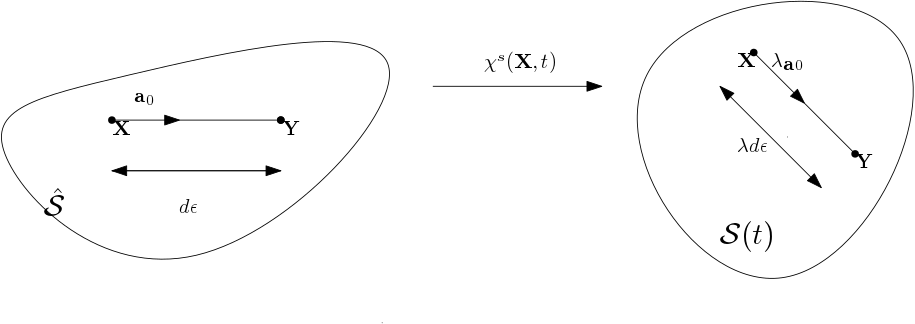
\includegraphics[scale=0.40]{./Solid_equations/Strain.png}
\caption{Deformation of a line element with length $d\epsilon$ into a line element with length $\lambda d \epsilon$}
\end{figure}

Strain is the relative change of location between two particles. Strain, strain rate and deformation is used to describe the relative motion of particles in a continuum. This is the fundamental quality that causes stress \cite{Richter2010}.

Observing two neighboring points \textbf{X} and \textbf{Y}. Let \textbf{Y} be described by adding and subtracting the point \textbf{X} and rewriting \textbf{Y} from the point \textbf{X} plus a distance $d\textbf{X}$   :
\begin{equation}
\textbf{Y} = \textbf{Y} + \textbf{X} - \textbf{X} = \textbf{X} + |\textbf{Y} - \textbf{X}| \frac{\textbf{Y} - \textbf{X}}{|\textbf{Y} - \textbf{X}|} = \textbf{X} + d\textbf{X}
\end{equation}

Let $d\textbf{X}$ be denoted by:
\begin{align}
d\textbf{X} =& d\epsilon \textbf{a}_0\\
d\epsilon =& |\textbf{Y} - \textbf{X}| \\
\textbf{a}_0 =& \frac{\textbf{Y} - \textbf{X}}{|\textbf{Y} - \textbf{X}|}
\end{align}
where $d\epsilon$ is the distance between the two points and $\textbf{a}_0$ is a unit vector 

We see now that $d\textbf{X}$ is the distance between the two points times the unit vector. \newline

A certain motion transform the points $\textbf{Y}$ and $\textbf{X}$ into the displaced positions $\textbf{x} = \chi^s(\textbf{X},t)$ and $\textbf{y} = \chi^s(\textbf{Y},t)$. Using Taylor`s expansion \textbf{y} can be expressed in terms of the deformation gradient:

\begin{align}
\textbf{y} =& \chi^s(\textbf{Y},t) = \chi^s(\textbf{X} + d\epsilon \textbf{a}_0,t) \\
=& \chi^s(\textbf{X},t) + d\epsilon F \textbf{a}_0 + \mathcal{O}(\textbf{Y}-\textbf{X}) 
\end{align}

where $\mathcal{O} (\textbf{Y}-\textbf{X})$ refers to the small error that tends to zero faster than $(\textbf{X} - \textbf{Y}) \rightarrow \mathcal{O}$. \newline

Setting $\textbf{x} = \chi^s(\textbf{X},t)$  It follows that:
\begin{align}
\textbf{y} - \textbf{x} =&  d\epsilon F \textbf{a}_0 + \mathcal{O}(\textbf{Y}-\textbf{X}) \\
=& F(\textbf{Y} - \textbf{X}) + \mathcal{O}(\textbf{Y}-\textbf{X}) 
\end{align}

Let the $\textbf{stretch vector}$ be $\lambda_{\textbf{a}0}$, which goes in the direction of $\textbf{a}_0$: 
\begin{equation}
\lambda_{\textbf{a}0}(\textbf{X},t) = F(\textbf{X},t)\textbf{a}_0 
\end{equation}

Looking at the square of $\lambda$:
\begin{align}
\lambda^2 &=  \lambda_{\textbf{a}0} \lambda_{\textbf{a}0} = F(\textbf{X},t)\textbf{a}_0 F(\textbf{X},t)\textbf{a}_0 \\
&= \textbf{a}_0 F^TF\textbf{a}_0 = \textbf{a}_0 C \textbf{a}_0
\end{align}

Introducing the right Cauchy-Green tensor:
 \begin{equation}
 C = F^TF
\end{equation}
Since $\textbf{a}_0 $ is just a unit vector, we see that C measures the squared length of change under deformation. We see that in order to determine the stretch one needs only the direction of $\textbf{a}_0$ and the tensor C.
C is also symmetric and positive definite $C = C^T$.  I also introduce the Green-Lagrangian strain tensor E:
\begin{equation}\label{eq:StrainTensor}
E = \frac{1}{2}(C - I) 
\end{equation}
which is also symmetric since C and I are symmetric. The Green-Lagrangian strain tensor E has the advantage of having no contributions when there is no deformations. Where the Cauchy-Green tensor gives the identity matrix for zero deformation.
		
\subsection{Stress}
While strain, deformation and strain rate only describe the relative motion of particles in a given volume, stress give us the internal forces between neighboring particles. Stress is responsible for deformation and is therefore crucial in continuum mechanics. The unit of stress is force per area.

Introducing the Cauchy stress tensor $\sigma_s$, which define the state of stress inside a material. The version of Cauchy stress tensor is defined by the material model used. 
If we use this tensor on an area, taking the stress tensor times the normal vector $\sigma_s \bold{n}$ we get the forces acting on that area.

Stress tensor defined from the Cauchy by the constitutive law of St. Venant-Kirchhoff hyperelastic material model: 
\begin{equation}
 \sigma_s = \frac{1}{J} F(\lambda_s (tr E)I + 2\mu_sE) F^T
\end{equation}

Using the deformation gradient and the Jacobian determinant, we get the first Piola-Kirchhoff stress tensor P:
\begin{equation}
 P = J \sigma F^{-T} 
\end{equation}
This is known as the \textit{Piola Transformation} and maps the tensor into a Lagrangian formulation which will be used when stating the solid equation.

Introducing the second Piola-Kirchhoff stress tensor S:
\begin{equation}
S = J F^{-1}\sigma F^{-T} = F^{-1} P = S^T 
\end{equation}
from this relation the first Piola-Kirchhoff tensor can be expressed by the second:
\begin{equation}
P = FS
\end{equation}

\chapter{Results from Renowned Scientists}\label{sec:bigboys}
\begin{figure}[H]
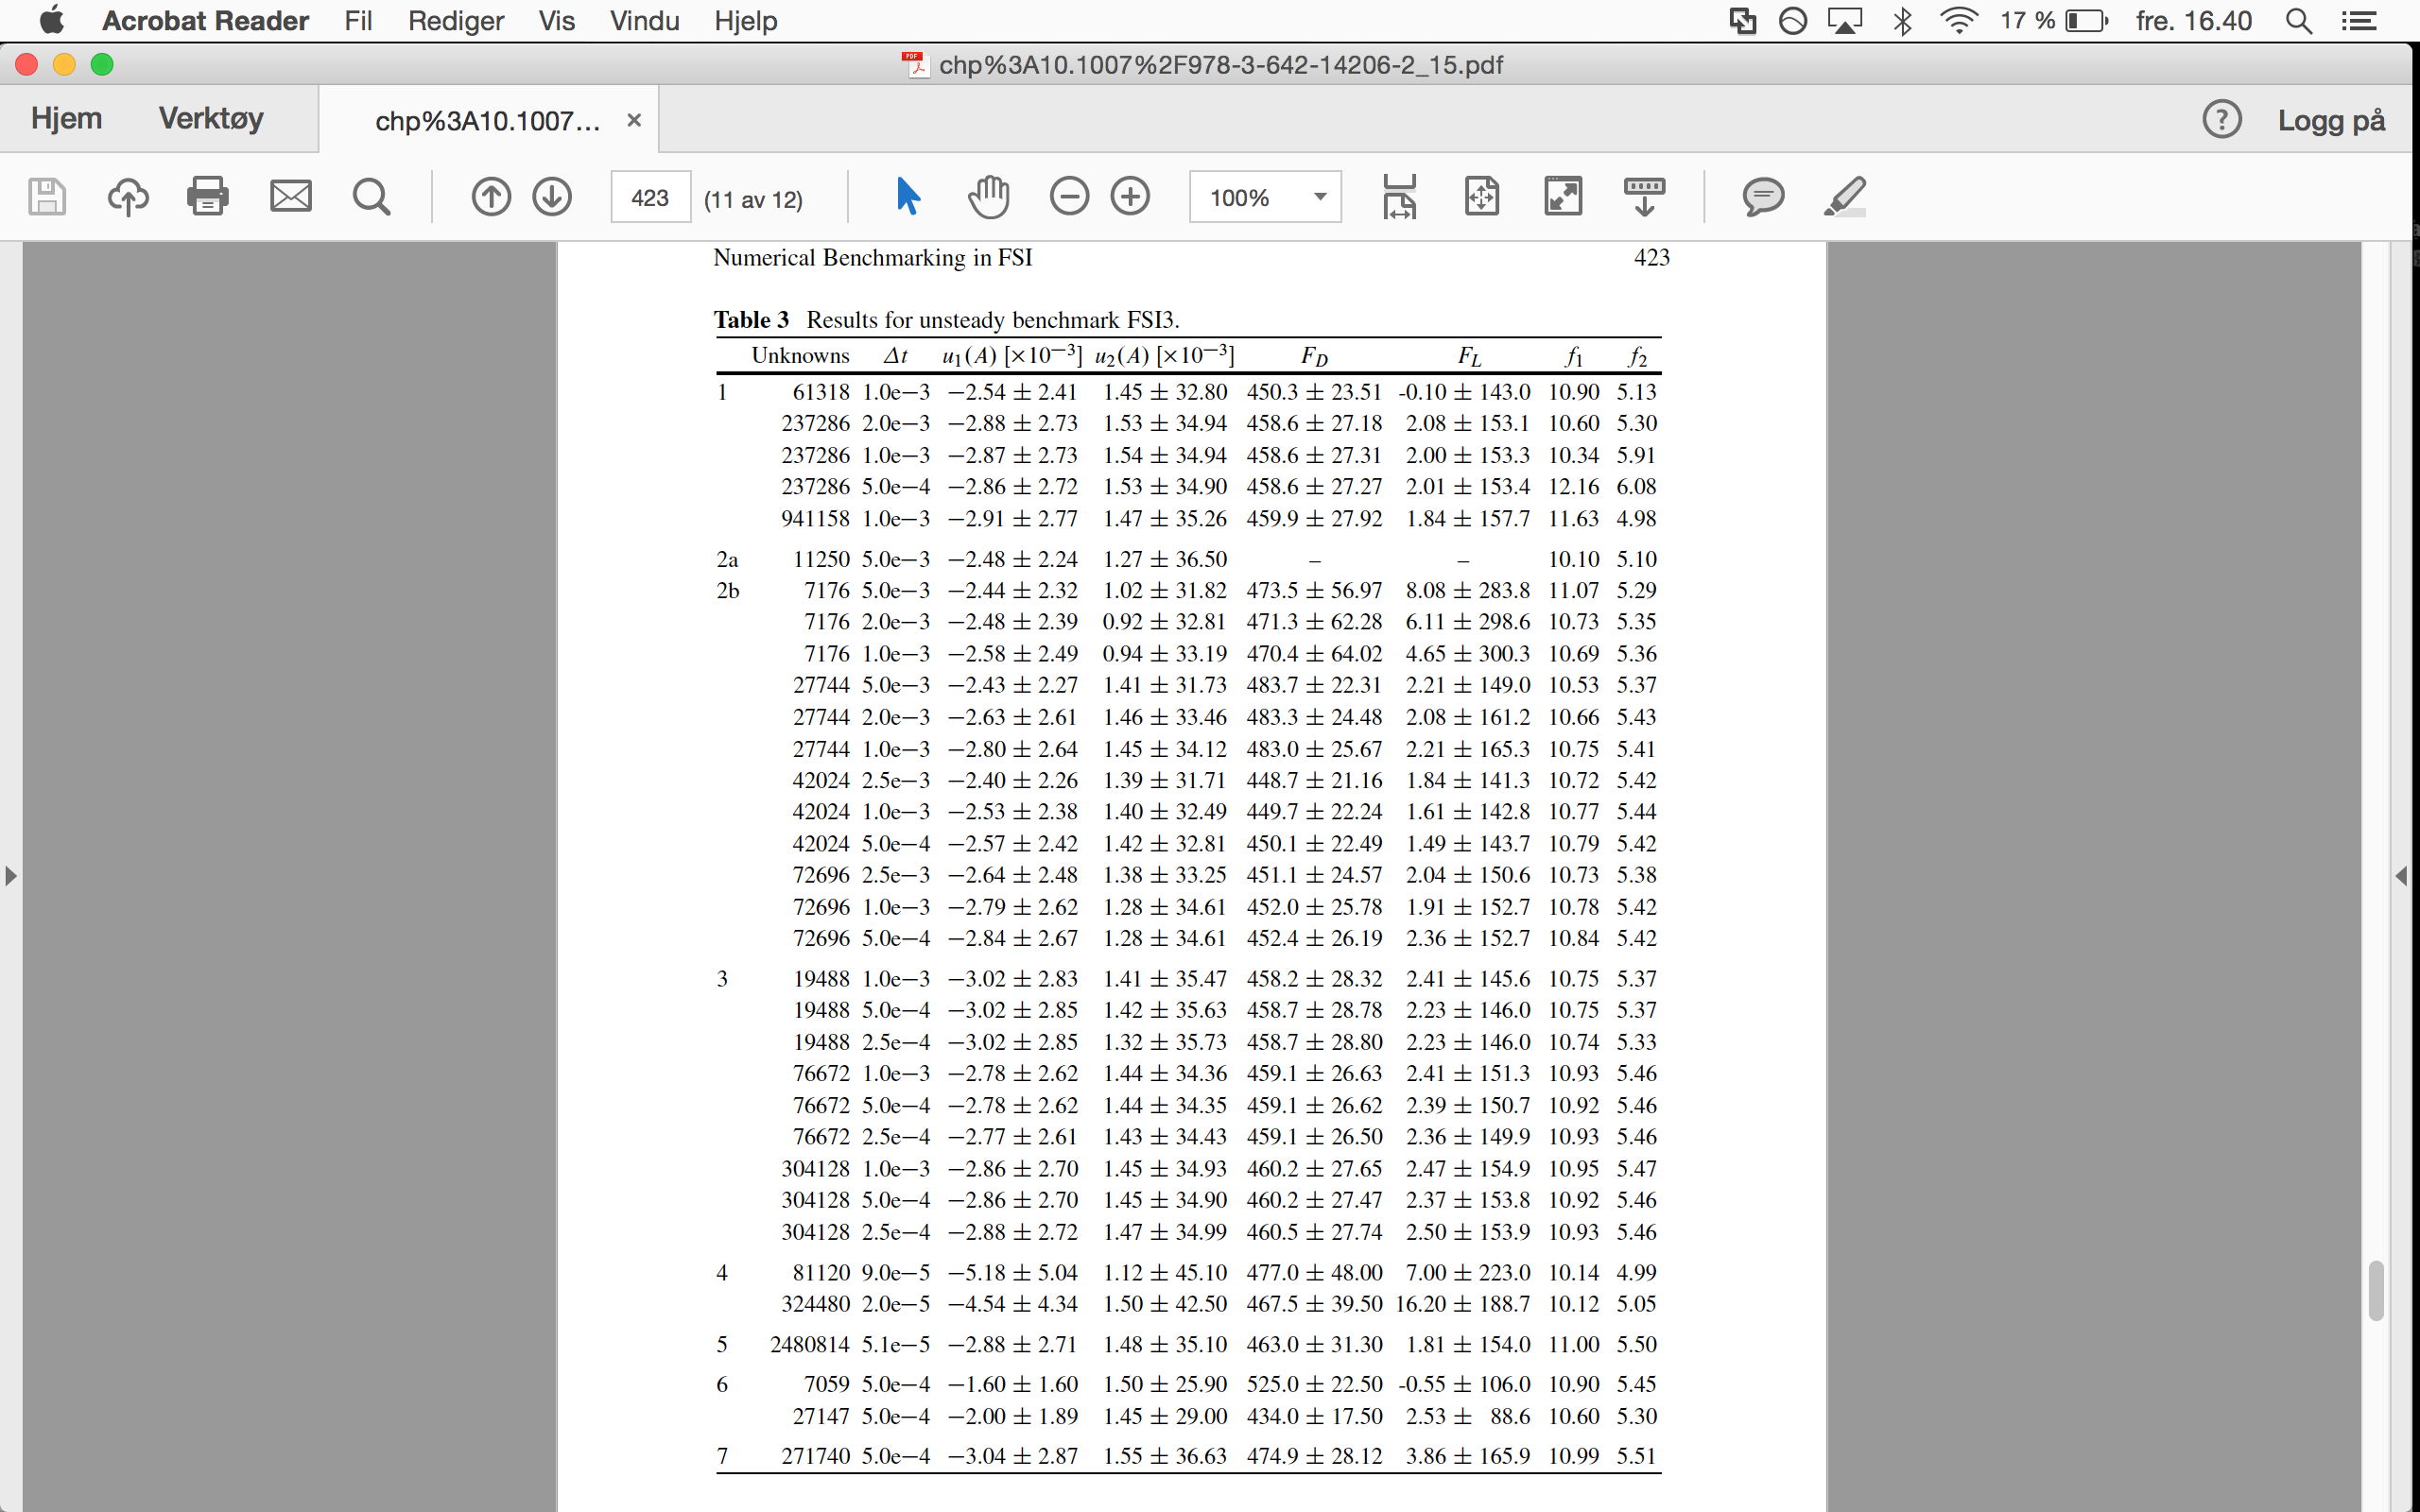
\includegraphics[scale=0.6,trim={12cm 0cm 16.3cm 5.5cm},clip]{./Appendix/BigBoyResults.png}
\caption{Results from different contributions in from the paper Turek et.al 2010 \cite{Turek2010}}
\end{figure}


\begin{comment}
\lstdefinelanguage{Python}{
 keywords={typeof, null, catch, switch, in, int, str, float, self},
 ndkeywords={boolean, throw, import},
 ndkeywords={return, class, if ,elif, endif, while, do, else, True, False , catch, def},
 ndkeywordstyle=\color{blue}\bfseries,
 identifierstyle=\color{black},
 sensitive=false,
 comment=[l]{\#},
 morecomment=[s]{/*}{*/},
 commentstyle=\color{purple}\ttfamily,
 stringstyle=\color{red}\ttfamily,
 backgroundcolor = \color{lightgray}
}
\end{comment}


\chapter{Implementation of Fluid Structure Interaction in FEniCS}
This Chapter shows the implementation of the FSI code in FEniCS \cite{FENICS}. FEniCS is platform used to solve partial differential equations. Code is written in python and FEniCS makes it easy to run efficient finite element code. \newline

The complete code consist of many hundreds of lines of code, and therefore only the most essential parts are covered. The code that has been added is added so that a reader with a minimal skill set in scientific computing and basic knowledge of the finite element method could implement a version of the code.



\section{Mappings}
The deformation gradient and the Jacobian is made using python functions. The deformation gradient python function takes in the deformation and returns the deformation gradient. Identity in FEniCS is a function that makes the identity matrix, with the size determined by a input value. The identity takes the length of the deformation function which for 2D cases is 2. grad is a built in FEniCS function that takes a vectorfunction and take the gradient.
\begin{python}\caption{Fenics code of deformation gradient and Jacobian}
def F_(d): """inputs deformation """
	return (Identity(len(d)) + grad(d))  """Returns the deformation gradient"""

def J_(d):
	return det(F_(d))
\end{python}


\section{Variational form}

The variational form can be written directly into FEniCS. A big advantage in FEniCS is that one can write all the forms and add them together to make the full variational form.
The vector functions and functions such as the displacement, velocity, and pressure, are written with a script n meaning at which time the function is valued. 
\begin{python}\caption{Deformation, velocity and pressure function described at three different timesteps }
d_["n"]  """deformation in the current timestep """
u_["n-1"] """velocity in the last timestep """
p_["n-2"] """pressure in the second last timestep """
\end{python}

theta is the value $\theta$ that determines the scheme.
k is the timestep $\Delta t$\\
$F_fluid_linear$ is the linear part of the variational form, and $F_fluid_nonlinear$ is the nonlinear part. Each part is assembled later when using newtonsmethod. 

Constant is a function in FEniCS that represents a constant value unknown at compile-time. Its value can be changed without the need to re-compilation of C++ code, which FEniCS utilizes.
$sigma_f$ and $sigma_f $ is the velocity and pressure parts of the fluid stress tensor.
grad and div are built-in functions in FEniCS that computes the gradient and divergence and given vector.
$dx_f$ denotes the fluid domain. 
$inv()$ is a built-in function in FEniCS outputs the inverse of the given matrix. 
psi, phi and gamma are the test functions.

\begin{python}
J_theta = theta*J_(d_["n"]) + (1 - theta)*J_(d_["n-1"]) 

F_fluid_linear = rho_f/k*inner(J_theta*(v_["n"] - v_["n-1"]), psi)*dx_f

F_fluid_nonlinear =  Constant(theta)*rho_f*\
inner(J_(d_["n"])*grad(v_["n"])*inv(F_(d_["n"]))*v_["n"], psi)*dx_f

F_fluid_nonlinear += inner(J_(d_["n"])*sigma_f_p(p_["n"], d_["n"])*\
inv(F_(d_["n"])).T, grad(psi))*dx_f

F_fluid_nonlinear += Constant(theta)*inner(J_(d_["n"])\
*sigma_f_u(v_["n"], d_["n"], mu_f)*inv(F_(d_["n"])).T, grad(psi))*dx_f

F_fluid_nonlinear += Constant(1 - theta)*inner(J_(d_["n-1"])*\
sigma_f_u(v_["n-1"], d_["n-1"], mu_f)*inv(F_(d_["n-1"])).T, grad(psi))*dx_f

F_fluid_nonlinear += \
inner(div(J_(d_["n"])*inv(F_(d_["n"]))*v_["n"]), gamma)*dx_f

F_fluid_nonlinear += Constant(1 - theta)*rho_f*\
inner(J_(d_["n-1"])*grad(v_["n-1"])*inv(F_(d_["n-1"]))*v_["n-1"], psi)*dx_f

F_fluid_nonlinear -= rho_f*inner(J_(d_["n"])*\
grad(v_["n"])*inv(F_(d_["n"]))*((d_["n"]-d_["n-1"])/k), psi)*dx_f
\end{python}

Fsolidlinear is the linear part of the variational form, and Fsolidnonlinear is the nonlinear part.
Piola1 is the first Piola-Kirchhoff stress tensor.
\begin{python}
delta = 1E10
F_solid_linear = rho_s/k*inner(v_["n"] - v_["n-1"], psi)*dx_s +\
delta*(1/k)*inner(d_["n"] - d_["n-1"], phi)*dx_s -\
delta*inner(Constant(theta)*v_["n"] + Constant(1-theta)*v_["n-1"], phi)*dx_s

F_solid_nonlinear = inner(Piola1(Constant(theta)*d_["n"] +\
Constant(1 - theta)*d_["n-1"], lamda_s, mu_s), grad(psi))*dx_s
\end{python}

The weighed delta is talked about in section \ref{Discretization}

\section{Newtons method implementation for solving Fluid structure interaction}
To solve a non-linear FSI problem, the newtons method has been implemented, ideas and code taken from from \cite{White2006}.

The derivative of the nonlinear variational parts is take with respect to dvp, which is the mixed function of displacement, velocity and pressure. -F is assembly of full variational form.


There is also an if test which only assembles the Jacobian the first and tenth time. This reuses the Jacobian to improve runtime, which is discussed in chapter \ref{runtime}. Lastly the the mpi line is when the code is running in parallel.
\begin{python}
def newtonsolver(F, J_nonlinear, A_pre, A, b, bcs, \
                dvp_, up_sol, dvp_res, rtol, atol, max_it, T, t, **monolithic):
    Iter      = 0  """ Setting initial values """
    residual   = 1  
    rel_res    = residual
    lmbda = 1

    while rel_res > rtol and residual > atol and Iter < max_it:
        if Iter % 10 == 0:
            A = assemble(J_nonlinear, tensor=A, form_compiler_parameters = {"quadrature_degree": 4})
            A.axpy(1.0, A_pre, True)
            A.ident_zeros()

        b = assemble(-F, tensor=b)

        [bc.apply(A, b, dvp_["n"].vector()) for bc in bcs]
        up_sol.solve(A, dvp_res.vector(), b)
        dvp_["n"].vector().axpy(lmbda, dvp_res.vector())
        [bc.apply(dvp_["n"].vector()) for bc in bcs]
        rel_res = norm(dvp_res, 'l2')
        residual = b.norm('l2')
        if isnan(rel_res) or isnan(residual):
            print "type rel_res: ",type(rel_res)
            t = T*T

        if MPI.rank(mpi_comm_world()) == 0:
            print "Newton iteration %d: r (atol) = %.3e (tol = %.3e), r (rel) = %.3e (tol = %.3e) " \
        % (Iter, residual, atol, rel_res, rtol)
        Iter += 1

    return dict(t=t)
\end{python}




	







\end{appendices}
%\newpage
%



\section*{Problem Defintion}
\subsection*{Domain}
The computational domain resembles the classic cfd benchmark with an added bar, with dimensions: \\
The box: L = 2.5, H = 0.41 \\
The bar: l = 0.35, h = 0.02 \\
The circle is positioned at (0.2, 0.2) making it 0.05 of center from bottom to top, this is done to induce oscillations to an otherwise laminar flow.\\
Boundary conditions:\\
The fluid velocity has a parabolic profile on the inlet that changes over time:\\

\begin{align*}
u(0,y) &= 1.5u_0 \frac{y(H-y)}{(\frac{H}{2})^2}  \\
u(0,y,t) &= u(0,y)\frac{1-cos(\frac{\pi}{2}t)}{2} \text{  for  } t<2.0 \\
u(0,y,t) &= u(0,y) \text{  for  } t \leq 2.0
\end{align*}

We set no slip on the "floor" and "ceiling" so to speak.\\
On the fluid solid interface the boundary conditions are set to:
$$  \sigma_f n_f = \sigma_s n_s \hspace{4mm} on  \hspace{2mm}\Gamma^0 (interface)   $$
In our variational form we leave this out and so implying that they are equal.

\subsection*{CSM test}
Parameters
\begin{table}[h]
\centering
\caption{My caption}
\label{my-label}
\begin{tabular}{|l|l|l|l|}
\hline
Parameters & CSM1 & CSM2 & CSM3 \\ \hline
$\rho_f[10^3 \frac{kg}{m^3}]$ & 1 & 1 & 1 \\ \hline
$\nu_f [10^{-3} \frac{m^2}{s}]$ & 1 & 1 & 1 \\ \hline
$u_0$ & 0 & 0 & 0 \\ \hline
$\rho_s[10^3 \frac{kg}{m^3}]$ & 1 & 1 & 1 \\ \hline
$\nu_s$ & 0.4 & 0.4 & 0.4 \\ \hline
$\mu_s[10^6 \frac{m^2}{s}]$ & 0.5 & 2.0 & 0.5 \\ \hline
$g $ & 2 & 2 & 2 \\ \hline
\end{tabular}
\end{table}

\newpage 

\subsection*{FSI test}
\begin{table}[ht]
\centering
\caption{Parameters}
\label{my-label}
\begin{tabular}{|l|l|l|l|}
\hline
Parameters & FSI1 & FSI2 & FSI3 \\ \hline
$\rho_f[10^3 \frac{kg}{m^3}]$ & 1 & 1 & 1 \\ \hline
$\nu_f [10^{-3} \frac{m^2}{s}]$ & 1 & 1 & 1 \\ \hline
$u_0$ & 0.2 & 1 & 2 \\ \hline
Re = $\frac{U d}{\nu_f}$ & 20 & 100 & 200 \\ \hline
$\rho_s[10^3 \frac{kg}{m^3}]$ & 1 & 10 & 1 \\ \hline
$\nu_s$ & 0.4 & 0.4 & 0.4 \\ \hline
$\mu_s[10^6 \frac{m^2}{s}]$ & 0.5 & 0.5 & 2 \\ \hline
\end{tabular}
\end{table}
Results: 
\begin{table}[h]
\centering
\caption{FSI 1}
\label{my-label}
\begin{tabular}{|l|l|l|l|l|l|l|}
\hline
Cells & Dofs & ux of A $[x10^{-3}]$ & uy of A $[x10^{-3}]$ & Drag & Lift & Spaces \\ \hline
2698 & 7095 & 0.0234594 & 0.797218  & 14.4963 & 0.915801 & P1-P1-P1 stab= 0.01 \\ \hline
2698 & 23563 & 0.02271 & 0.80288 & 14.1736 & 0.787891 & P2-P2-P1 \\ \hline
2698 & 23563 & 0.00581116 & 0.000000738678  & 12.07 & 0.02345 & P2-P2-P1 without weighting \\ \hline
10792 & 92992 & 0.0227341 & 0.808792 & 14.1855 & 0.801044 & P2-P2-P1 \\ \hline
43168 & 369448 & 0.227352 & 0.812595 & 14.227 & 0.797242 & P2-P2-P1 \\ \hline
\textbf{ref} & \textbf{ref} & \textbf{0.0227} & \textbf{0.8209} & \textbf{14.295} & \textbf{0.7638} & \textbf{ref} \\ \hline
\end{tabular}
\end{table}
In my monolithic 






\bibliographystyle{plain}
\bibliography{Master_cites}


\end{document}